\documentclass[11pt,a4paper]{article}
\usepackage{fontspec}
\setmainfont{Source Serif 4}[Path=/home/claude/ref/fonts/, UprightFont=SourceSerif4-Regular.ttf, BoldFont=SourceSerif4-Semibold.ttf, ItalicFont=SourceSerif4-It.ttf]
\setmonofont{IBM Plex Mono}[Path=/home/claude/ref/fonts/, UprightFont=IBMPlexMono-Regular.ttf, BoldFont=IBMPlexMono-Medium.ttf, Scale=0.88]
\usepackage[a4paper,margin=2.4cm]{geometry}
\usepackage{amsmath}
\usepackage{graphicx,booktabs,float,caption,array,xcolor,longtable}
\usepackage{xurl}
\usepackage[hidelinks]{hyperref}
\usepackage[round]{natbib}
\usepackage{setspace}
\setstretch{1.08}
\renewcommand{\topfraction}{0.9}
\renewcommand{\bottomfraction}{0.8}
\renewcommand{\textfraction}{0.1}
\renewcommand{\floatpagefraction}{0.75}
\setlength{\parindent}{0pt}
\setlength{\parskip}{0.55em}
\captionsetup{font=small,labelfont=bf}
\setlength{\bibsep}{3pt}
\urlstyle{same}
\hypersetup{pdftitle={What Each Constituency Signs: The Geography of UK Parliament Petitions},pdfauthor={Dr Tristan Hotham}}

\begin{document}
\begin{center}
{\Large\bfseries What Each Constituency Signs: The Geography of UK Parliament Petitions, 2024 to 2026\par}
\vspace{1.2em}
{\large Dr Tristan Hotham\par}
\vspace{0.3em}
{\small Independent researcher\\
ORCID: 0000-0003-4931-9349\\
DOI: https://doi.org/10.5281/zenodo.24104518\par}
\vspace{0.8em}
2026
\end{center}

\begin{quote}
\small
\begin{center}\textbf{Abstract}\end{center}
Parliamentary e-petitions record where their signatories live, which turns every petition into a map of public concern. This paper analyses the geography of the 734 petitions to the UK Parliament elected in 2024 that reached about 3,000 signatures by 2026, using 30,338,613 signatures counted in all 650 constituencies. Following an analysis plan written before any outcome was computed, I measure each petition's over- and under-signing with empirical Bayes location quotients and test four expectations. First, every one of the 734 petition maps is spatially clustered (median Moran's $I$ = 0.48; shuffled seats give $-$0.00). Second, petitions about a particular place are far more concentrated than national ones: allowing for size, their excess dissimilarity is 189\% higher (95\% CI 71 to 389), though only ten such petitions exist. Third, seat profiles share a low-dimensional structure: two components hold 30\% of the variation, the first aligned with graduate, younger and more diverse seats against older, whiter seats with a higher Reform UK vote, and both are stable across petitions created in different periods (split-half $r$ = 0.96 and 0.96). Fourth, 2024 vote shares explain a median 26\% of a petition's seat map, less than census composition in England and Wales (31\%). EU petitions are under-signed where Reform UK polled strongly in every check; the planned association between immigration petitions and the Reform UK vote is fragile because the family pools petitions with opposite aims. The results describe places, not people.

\textbf{Keywords:} e-petitions; political participation; electoral geography; constituencies; spatial autocorrelation; House of Commons
\end{quote}

\section{Introduction}\label{sec:intro}
Since 2015 the House of Commons and the government have run a joint e-petitions site. Any UK resident or British citizen can start or sign a petition, giving a name, an email address and, for UK residents, a postcode. Petitions that pass 10,000 signatures receive a government response and those that pass 100,000 are considered for debate. Popular petitions draw very large numbers of signatures, although few lead to specific policy action \citep{lestonbandeira2019,asher2019}. Less noticed is a by-product of its design: because each signature carries a postcode, the site publishes a running count of signatures for every Westminster constituency. Each petition is therefore also a map.

This paper treats those maps as data on the geography of public concern. It asks four questions. How far does each petition's geography depart from the overall map of petition signing, and does that departure cluster in space? Which kinds of petition are most and least geographic? Do constituencies have stable ``signature personalities'', a few dimensions that summarise what each seat over-signs? And how closely do petition geographies follow the 2024 general election vote, compared with the demographic make-up of seats? The data are the 734 petitions to the Parliament elected in July 2024 that had reached about 3,000 signatures when the data were retrieved in 2026. They carry 93\% of all signatures given to the 17,201 petitions of the Parliament, of which 9,057 were rejected by the Petitions Committee's staff.

The study makes three contributions. First, it supplies a systematic, constituency-level description of what the public petitions about and where, on the boundaries introduced in 2024, with all 650 seats and a measure that separates a petition's geography from the overall propensity of a seat to sign anything. Second, it tests, in a design fixed in a written plan before any outcome was computed, whether petition geographies are structured: clustered in space, concentrated for local causes, organised along a small number of stable dimensions, and related to the vote. Third, it shows where that structure lies: two broad dimensions that resemble the education and age divides found in recent British electoral geography \citep{jenningsstoker2016,goodwinheath2016}, with the vote adding less than census composition.

The answers are clear for the first three questions and more qualified for the fourth. Every petition map is clustered. Local causes are by far the most concentrated, as expected, although there are only ten of them. Seats differ along two dominant and very stable dimensions. Vote shares account for about a quarter of a typical petition's map, roughly as much as knowing the region and less than four census shares; and of the two planned directional tests, the link between EU petitions and a lower Reform UK vote is robust while the link between immigration petitions and a higher Reform UK vote is not, because the immigration family contains petitions with opposite aims.

The design is descriptive and correlational. A constituency is not a person, and the maps say nothing directly about who signed \citep{robinson1950}. The paper proceeds as follows. Section~\ref{sec:lit} reviews research on e-petitions and on the geography of political behaviour. Section~\ref{sec:data} describes the data and Section~\ref{sec:design} the measures, hypotheses and models. Section~\ref{sec:results} reports the results and Section~\ref{sec:robust} the checks. Section~\ref{sec:disc} discusses the findings and their limits, and Section~\ref{sec:conc} concludes.

\section{Background and literature}\label{sec:lit}
\subsection{E-petitions in the UK}
Petitioning Parliament is among the oldest forms of political participation in Britain, but its online form is recent. The Downing Street e-petitions site (2006 to 2010) was followed by the government's own site and, from 2015, by the joint system run with the House of Commons Petitions Committee. Studies of the earlier systems established their basic dynamics. \citet{wright2012} assessed the Downing Street site against Smith's framework of ``democratic goods''; \citet{wright2016} showed that petitioners themselves define success more broadly than policy change. \citet{bochel2013} compared five petitions systems and the UK government's e-petitions site and argued that petitions can be a meaningful channel of participation within representative democracy.

Research on the current system has focused on its roles and its effects on Parliament. \citet{lestonbandeira2019} identified four roles of parliamentary petitions (linkage, campaigning, scrutiny and policy) and found that most petitions are rejected and few lead to concrete action, but that their main value lies in public engagement. \citet{asher2019} studied Twitter conversations around petitions debated in Westminster Hall and found mixed views of the process. \citet{matthews2021} interviewed MPs and found many indifferent or hostile to e-petitions, partly because they worry that petitions bypass the constituency link. That concern makes the constituency geography of petitions directly relevant: if petitions are signed in recognisable places, MPs can read them as signals from their own seats.

A second strand studies signing as a large-scale behaviour. \citet{hale2013} and \citet{yasseri2017} analysed the growth of thousands of UK petitions and showed that most never reach the thresholds for a response or a debate and that a petition's fate is largely settled within its first day or two; \citet{margetts2016} built a broader account of ``political turbulence'' from such trace data. \citet{hagen2016} related the popularity of US We the People petitions to their language. German studies of the Bundestag system examined who signs and how signers spread across petitions \citep{jungherr2010,puschmann2017} and whether online petitioning reduces participatory inequality, finding that it does not \citep{escher2017}; \citet{riehm2014} compared electronic petitioning systems across Europe.

\subsection{Who signs, and the geography of participation}
Signing a petition is one of the easiest political acts, often discussed under the label of ``clicktivism'' \citep{halupka2014}. Low cost does not mean equal participation: \citet{schlozman2010} showed that online acts such as signing petitions were as stratified by socioeconomic status as their offline equivalents. Differences between places in who signs are therefore expected, and any analysis of petition geography must separate a petition's own map from the general level of signing in each seat. This paper does so by measuring each seat's share of a petition against its share of all petition signatures.

The geography of British political behaviour has a long literature. \citet{agnew1987} argued that place mediates political attitudes through local contexts, and \citet{johnstonpattie2006} documented the persistent geography of British voting. More recent work has emphasised divides by education, age and place type: \citet{jenningsstoker2016} described a ``bifurcation'' between a cosmopolitan and a provincial England, and aggregate studies of the 2016 referendum found Leave support sharply divided by education \citep{goodwinheath2016,beckeretal2017}. If petitions express the same divides, their geographies should be structured along similar lines.

\subsection{Petitions as a record of issue salience}
Petitions are also a record of what the public thinks matters. Research on political attention treats the problems that governments and legislatures address as a scarce agenda shaped by public priorities \citep{jonesbaumgartner2005}, and research on responsiveness asks whether policy follows the public's preferences and their changes \citep{sorokawlezien2010}. Both literatures usually measure the public side with national surveys. Petitions differ in three ways: they are self-generated rather than prompted by a question, they are specific (a named drug, a rail line, a tax threshold) rather than broad categories, and they are recorded continuously and locally. The cost is that they capture intensity among a self-selected minority, not the distribution of opinion. Treating them as a geography of salience, rather than of opinion, matches what they measure: where enough people cared enough to act.

\subsection{Mapping petitions}
The closest predecessor is \citet{vidgen2020}, who applied topic models to 10,950 petitions submitted to the UK government between 2015 and 2017, traced their popularity over time and mapped where signatories lived, grouping constituencies into six clusters by the issues they supported. The present paper builds on that work in four ways. It covers the Parliament elected in 2024 and the new constituency boundaries; it measures over-signing with a location quotient shrunk towards the national pattern, so that small seats cannot dominate by chance \citep{claytonkaldor1987}; it tests pre-specified hypotheses about clustering, local causes, stability and the vote; and it compares the explanatory power of vote shares, region and census composition petition by petition.

\subsection{What is new here}
To the best of my knowledge this is the first study of the constituency geography of the post-2024 petitions, the first to test petition geography against the 2024 vote, and the first to show that the main dimensions of petition geography are stable across independent sets of petitions. It contributes to the literature on e-petitions a measure of where concerns come from, and to political geography a large set of revealed issue preferences recorded seat by seat between elections.

\section{Data}\label{sec:data}
\subsection{Petitions}
The petitions site \citep{petitions2026} publishes, for each petition, its title (``action''), a background statement, its state (open, closed or rejected), dates, and the signature count; for petitions with signatures it also publishes counts by constituency, region and country. The list used here contains all 17,201 petitions created between 2024-10-30 and 2026-11-08 (2,167 open, 5,977 closed and 9,057 rejected). Constituency counts were retrieved for the 734 petitions with about 3,050 or more signatures (the smallest included has 3,052; the largest excluded 3,033). Together they hold 30,882,864 signatures, of which 30,338,613 are assigned to a constituency; the rest come from abroad or unmatched postcodes (for the median petition, 98.7\% of signatures are assigned). 89 petitions passed 100,000 signatures and 450 passed 10,000. The site does not tag topics, so I coded them (Section~\ref{sec:topics}).

\subsection{Constituencies, votes and census shares}
Constituencies are the 650 seats used from the 2024 general election. Two geographies are used: the Open Innovations hexagon layout \citep{openinnovations2023}, which gives every seat equal area for display, and simplified ONS boundaries, used to define neighbours. Vote shares at the 2024 general election, Census 2021 shares (aged 65 and over, holding a degree or higher, health not good, and White) and the simplified boundaries come from the voteReproject package \citep{horan2025}, which compiles House of Commons Library results and ONS census and boundary data for the 2024 seats. Census shares are available for the 575 seats in England and Wales. Electorates were not available, but the 2023 boundary review placed nearly every seat's electorate within 5\% of a common quota, so raw signature totals are close to rates per elector; 2024 valid votes serve as an alternative denominator.

\subsection{Topic families}\label{sec:topics}
Petitions were sorted into fifteen families by ordered keyword rules applied to the action text (and the background if the action matched nothing), written before any outcome was computed. Every one of the 734 petitions was then read by eye, and 123 (16.8\%) were moved by hand; the overrides are listed in the replication files. Most corrections moved petitions about particular groups (for example Hong Kong British Nationals (Overseas) or Ukrainians) from the ``local causes'' rule to immigration, support for children with special educational needs from health to schools, petitions about gender identity to equality, and petitions about the European Convention on Human Rights to crime, justice and rights. Local causes are petitions whose action names a particular part of the UK: ten petitions about Cornwall, the Scottish Parliament, the London Mayor, Northern Ireland veterans, the A1 in the North of England, independence referendums in Scotland and Wales, and the rail link between Oxford and Cambridge. Table~\ref{tab:fam} lists the families. The families are broad and some (immigration, the EU) contain petitions with opposite aims, a point that matters in Section~\ref{sec:votes}.

\begin{table}[tbp]\centering\small\caption{Topic families. $D$: index of dissimilarity (\% of signatures that would have to move to match the overall map); $I$: Moran's $I$; top 10: share of signatures from the ten most over-signing seats; excess $D$: geometric mean of $D$ minus its sampling expectation, adjusted for log size and open status (model in Section~\ref{sec:design}), with 95\% CI. Medians unless stated.}\label{tab:fam}\footnotesize\setlength{\tabcolsep}{3pt}\begin{tabular}{lrrrrrl}\toprule Family & $N$ & Sig. (000) & $D$ (\%) & $I$ & Top 10 (\%) & Excess $D$ (\%)\\\midrule
Local causes & 10 & 396 & 77.9 & 0.61 & 44.8 & 41.2 [24, 71]\\
Immigration and asylum & 54 & 3,172 & 37.9 & 0.43 & 8.7 & 18.2 [14, 23]\\
International affairs & 33 & 828 & 32.7 & 0.44 & 7.4 & 17.0 [12, 23]\\
Environment, energy and planning & 51 & 1,416 & 32.4 & 0.51 & 11.6 & 23.8 [19, 29]\\
Transport and roads & 42 & 624 & 31.4 & 0.53 & 9.5 & 17.9 [14, 22]\\
Other & 19 & 289 & 30.7 & 0.48 & 12.6 & 18.7 [13, 27]\\
Health and care & 121 & 2,787 & 27.2 & 0.44 & 8.3 & 15.9 [14, 18]\\
Schools and children & 66 & 1,935 & 25.0 & 0.51 & 7.3 & 16.6 [15, 19]\\
Crime, justice and rights & 55 & 1,890 & 24.8 & 0.47 & 7.0 & 14.7 [12, 18]\\
Equality and identity & 25 & 653 & 22.7 & 0.43 & 6.1 & 13.0 [10, 16]\\
Money, work and pensions & 100 & 2,961 & 21.6 & 0.48 & 5.1 & 11.4 [10, 13]\\
Online life and technology & 30 & 4,725 & 19.7 & 0.48 & 5.2 & 10.2 [8, 13]\\
Animals and fireworks & 82 & 3,143 & 19.4 & 0.50 & 5.4 & 10.8 [9, 12]\\
Brexit and the EU & 12 & 371 & 17.4 & 0.44 & 3.7 & 8.4 [7, 9]\\
Elections and democracy & 34 & 5,695 & 15.8 & 0.54 & 3.9 & 8.4 [7, 10]\\
\bottomrule\end{tabular}\end{table}

\section{Research design}\label{sec:design}
\subsection{Analysis plan}
The plan (hypotheses, measures, models, checks and what would count against each hypothesis) was written in the study notes before any seat-level petition measure was computed, and is reproduced in the replication files. Results are reported as planned; analyses added afterwards are labelled exploratory.

\subsection{Measures}
Let $S_{pc}$ be the signatures for petition $p$ in constituency $c$, $T_c=\sum_p S_{pc}$ the seat's total over all petitions, $T_p=\sum_c S_{pc}$ and $T=\sum_{p,c}S_{pc}$. The expected count under no geography beyond overall activity is $E_{pc}=T_pT_c/T$ and the raw location quotient is $S_{pc}/E_{pc}$. Raw quotients are noisy where expected counts are small, so the main measure is an empirical Bayes estimate \citep{claytonkaldor1987}: for each petition a gamma prior with mean one and shape $\alpha_p$ estimated by the method of moments from the dispersion of raw quotients, giving the posterior mean $(S_{pc}+\alpha_p)/(E_{pc}+\alpha_p)$. Its logarithm is the petition's map.

Concentration is measured with the index of dissimilarity \citep{duncan1955}, $D_p=\tfrac12\sum_c|S_{pc}/T_p-T_c/T|$, the share of a petition's signatures that would have to move for its map to match the overall map of petition signing. Because sampling alone produces some dissimilarity, I subtract the mean $D$ of 50 multinomial draws with the same total (``excess $D$''). Clustering is measured with Moran's $I$ \citep{moran1950,anselin1995} of the log quotient over contiguity neighbours (polygons touching within about 250 metres, row-standardised; the two island seats without a land neighbour are linked to their nearest seat), with a permutation $p$-value from 199 random relabellings.

\subsection{Hypotheses and models}
\textbf{H1 (clustering).} Petition maps are spatially clustered: the median Moran's $I$ is positive and most petitions are significant at 5\%.

\textbf{H2 (local causes).} Local causes are more concentrated than national petitions. Model: OLS of log excess $D$ (floored at 0.005) on a local-cause indicator, log $T_p$ and an indicator for petitions still open, with HC3 errors \citep{mackinnon1985}.

\textbf{H3 (personalities).} Seat profiles have a low-dimensional structure that is stable over time. I run a principal component analysis \citep{jolliffecadima2016} of the $650\times734$ matrix of log quotients (columns standardised), report the variance shares, and recompute it separately for the petitions created before and after the median creation date; stability is the correlation of seat scores on matched components across the two halves. Seats are also grouped by $k$-means on the first five component scores, with $k$ chosen from 3 to 8 by the average silhouette width \citep{rousseeuw1987}.

\textbf{H4 (votes).} Petition geography follows the 2024 vote. (a) For each petition, the $R^2$ of an OLS regression of its log quotients on the 2024 shares of the Conservatives, Labour, the Liberal Democrats, Reform UK, the Greens and the SNP plus Plaid Cymru in the 632 seats of Great Britain, compared with region fixed effects alone and, in England and Wales, with the four census shares. (b) For each family, the seat's log family quotient (family signatures over family expected count) regressed on the five GB-wide party shares and the four census shares, all standardised, with region fixed effects and HC3 errors in the 575 seats of England and Wales. Models are estimated with statsmodels \citep{seabold2010}. Directional expectations: immigration petitions over-signed where Reform UK polled well; EU petitions under-signed where Reform UK polled well and over-signed where the Liberal Democrats and Greens did. Other coefficients are two-sided and descriptive. Coefficients are reported as the percentage change in the family quotient per standard deviation of the regressor.

\subsection{Checks}
Placebos: Moran's $I$ and vote $R^2$ with seat labels permuted (P1); and a reliability check (P2): groups of near-identical petitions should have highly correlated maps if the maps are signal rather than noise. Alternative specifications: raw rather than shrunk quotients; a petition-weighted denominator (the mean of each seat's share across petitions, which stops the largest petitions dominating $T_c$); 2024 valid votes as the denominator; dropping the five largest petitions; petitions with 10,000 or more signatures only; six-nearest-neighbour weights; keyword rules without the manual overrides; region-clustered errors (12 clusters, $t$ with 11 degrees of freedom; \citealt{cameronmiller2015}); leaving out each region, London, and Wales.

\subsection{Threats to inference}
The maps are aggregates of self-selected signers. Campaigns, local media and social networks can concentrate signing in a place for reasons unrelated to its residents' general views. Postcodes are self-reported. Petitions still open were still collecting. The composition of signers is unknown, so associations with vote shares and census shares are ecological \citep{robinson1950}. None of these threatens the descriptive findings, but they bound the interpretation of the associations.

\section{Results}\label{sec:results}
\subsection{What the maps look like}
Figure~\ref{fig:cases} shows six maps on a common scale. The largest petition, ``Call a General Election'' (3,084,711 signatures), departs little from the overall map ($D$ = 8\%). A local cause, ``Grant Cornwall nation status'', drew 67 times its expected share in Truro and Falmouth and 64 times in St Ives ($D$ = 69\%). In between, ``Don't change inheritance tax relief for working farms'' is strongest in rural English seats and Orkney and Shetland, ``Apply for the UK to join the European Union as a full member as soon as possible'' in Cambridge, Hornsey and Friern Barnet and Edinburgh North and Leith, and ``Introduce offshore detention/mass deportation for illegal migrants'' in Great Yarmouth (3.1 times). Seats also differ in overall activity, from 9,446 signatures across all petitions in Na h-Eileanan an Iar to 65,942 in Rayleigh and Wickford; per 2024 vote, activity correlates $-$0.66 with the degree share and 0.65 with the share in poor health in England and Wales, which is why each map is measured against the seat's own activity.

\begin{figure}[tbp]\centering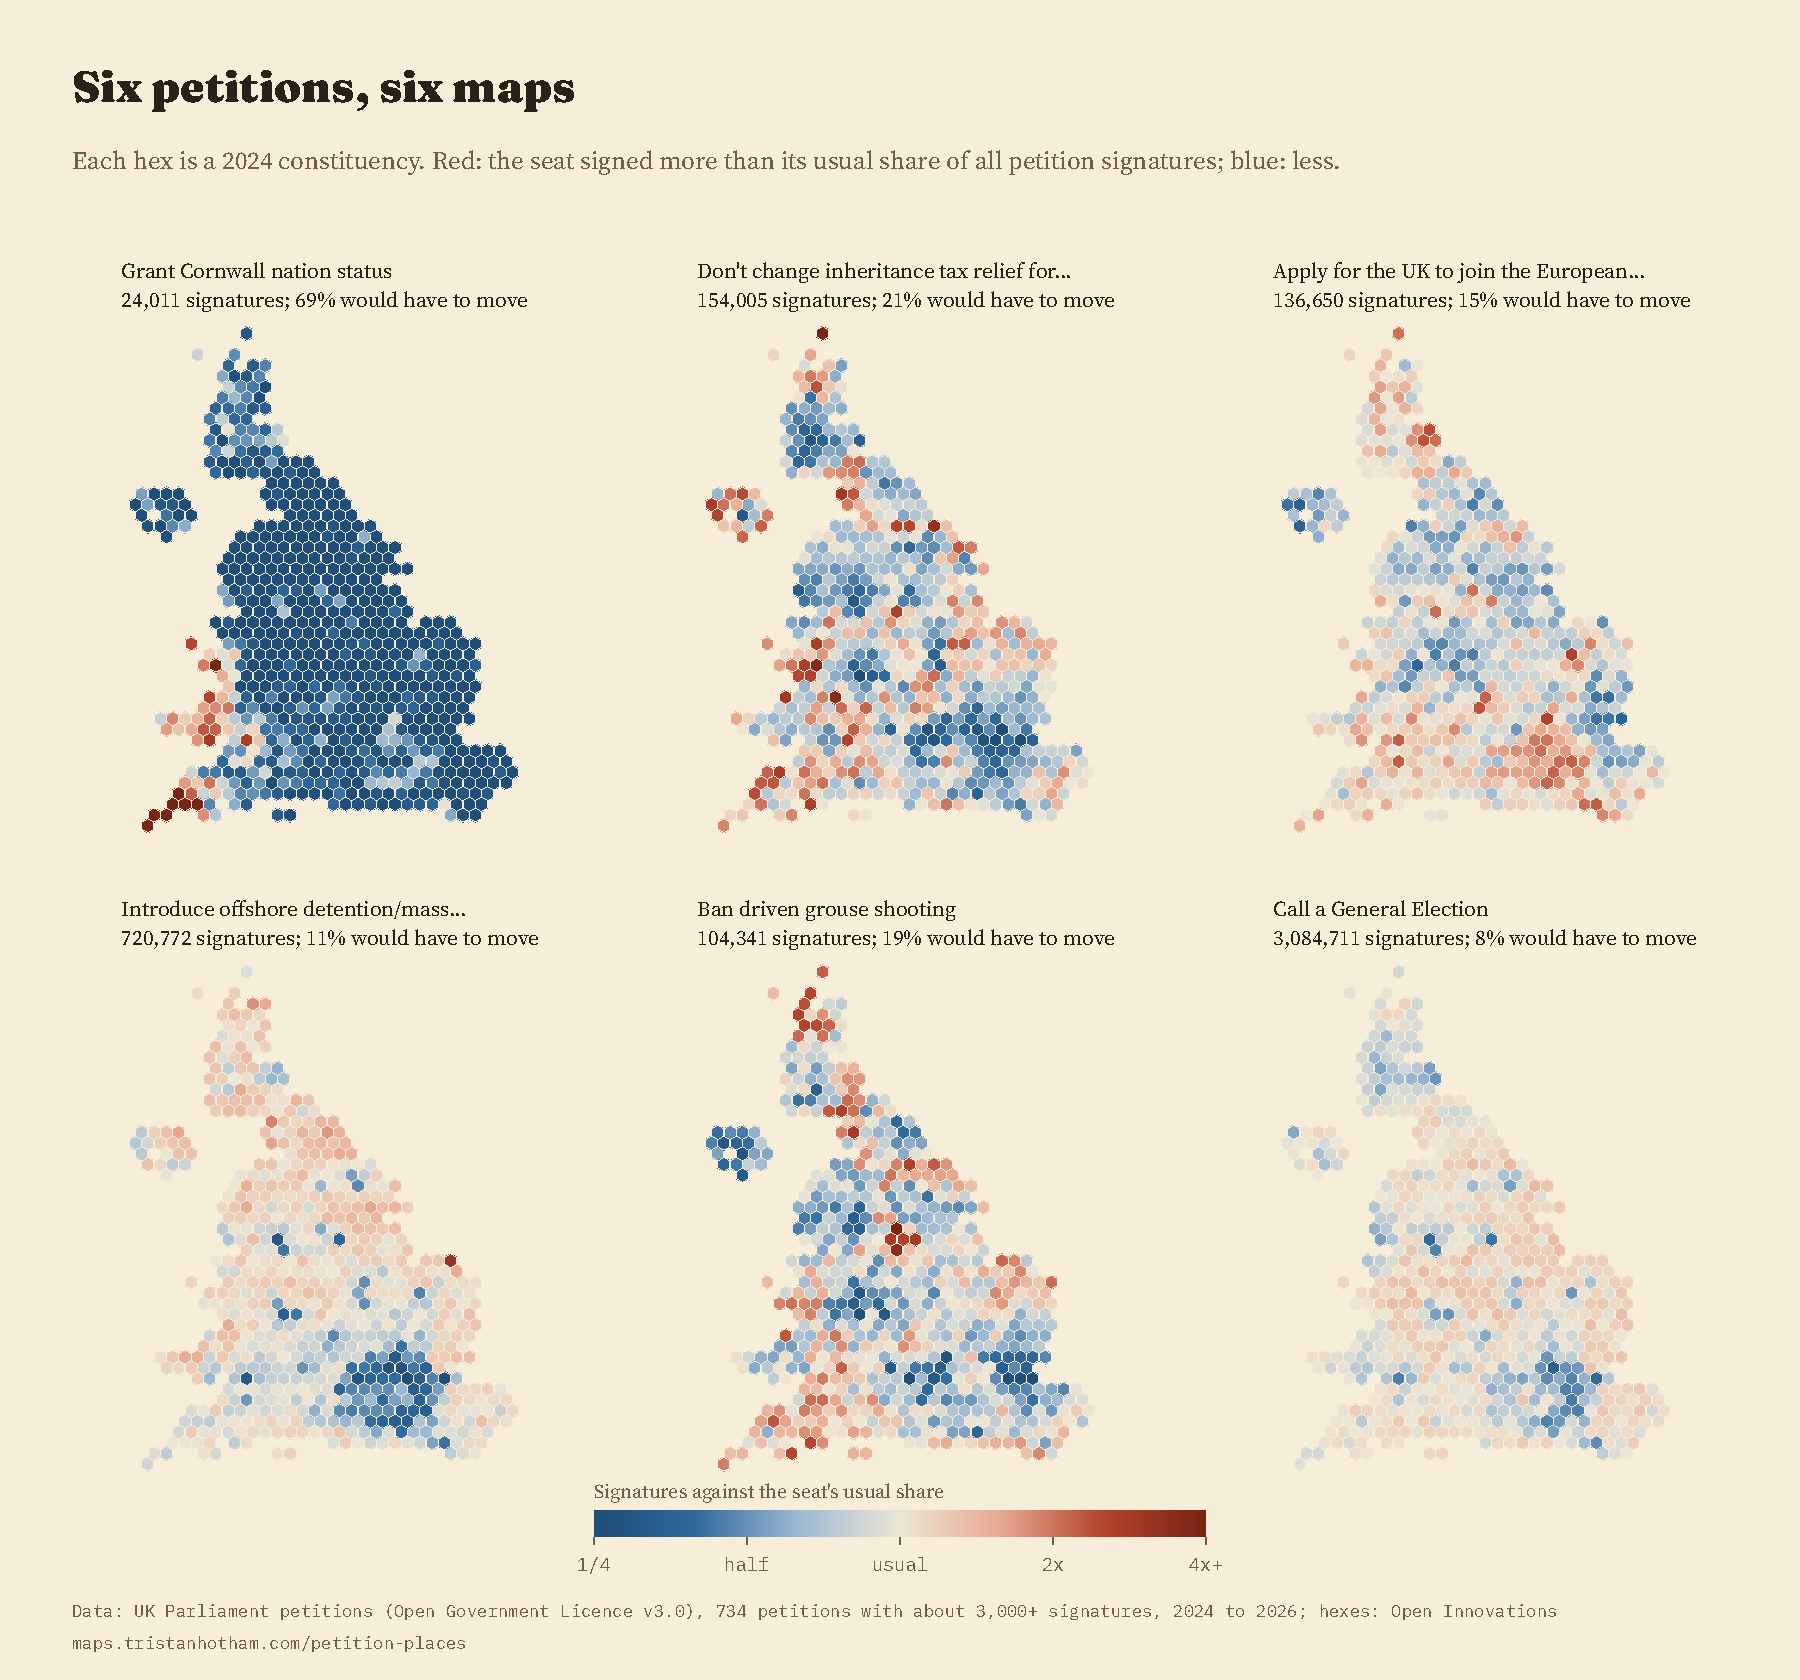
\includegraphics[width=\textwidth]{f_cases.pdf}\caption{Six petition maps. Each hexagon is a 2024 constituency, coloured by the empirical Bayes location quotient (log scale, clipped at a quarter and four times).}\label{fig:cases}\end{figure}

\subsection{H1: petition maps are clustered}
All 734 of the 734 petition maps are significantly clustered at the 5\% level (permutation tests). The median Moran's $I$ is 0.48 (interquartile range 0.37 to 0.60; minimum 0.04, maximum 0.92). With seat labels permuted it is $-$0.00 (Figure~\ref{fig:moran}). The typical petition has a dissimilarity of 24\% (14\% above sampling noise), and its ten most over-signing seats supply 6.5\% of its signatures, against 1.5\% if signatures followed seat numbers evenly. H1 is supported.

\begin{figure}[tbp]\centering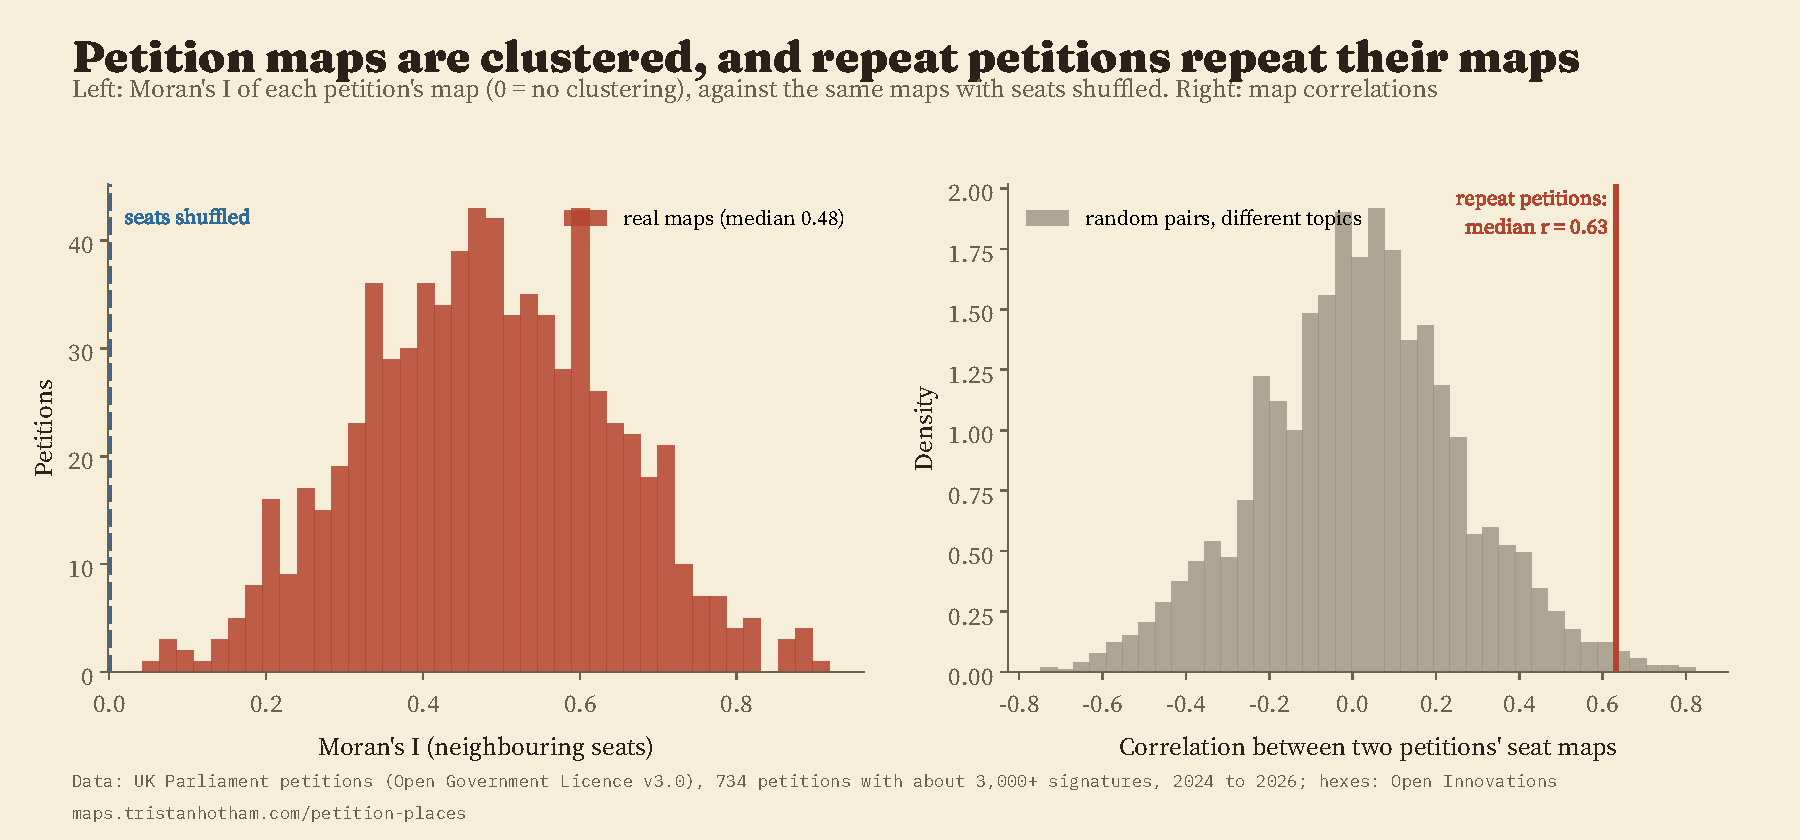
\includegraphics[width=\textwidth]{f_moran.pdf}\caption{Left: Moran's $I$ of the 734 petition maps, with the median under permuted seat labels (dashed). Right: correlations between the maps of near-identical petitions (median, red line) and between random pairs of petitions from different families (grey).}\label{fig:moran}\end{figure}

\subsection{H2: local causes are the most concentrated}
Figure~\ref{fig:family} and Table~\ref{tab:fam} compare families. The median local cause has $D$ = 78\%, against 24\% for all other petitions, and draws 45\% of its signatures from ten seats (others: 6.4\%). In the planned model (Table~\ref{tab:h2}), allowing for petition size and open status, local causes have 189\% higher excess dissimilarity (95\% CI 71 to 389, $N$ = 734 petitions, 10 local). Among national families, immigration petitions are the most concentrated (median $D$ 38\%) and petitions about elections and democracy the least (16\%). H2 is supported, with the caveat that it rests on ten petitions; among petitions of 10,000 or more signatures only six are local and the interval includes zero (110\%, CI $-$5 to 365).

\begin{figure}[tbp]\centering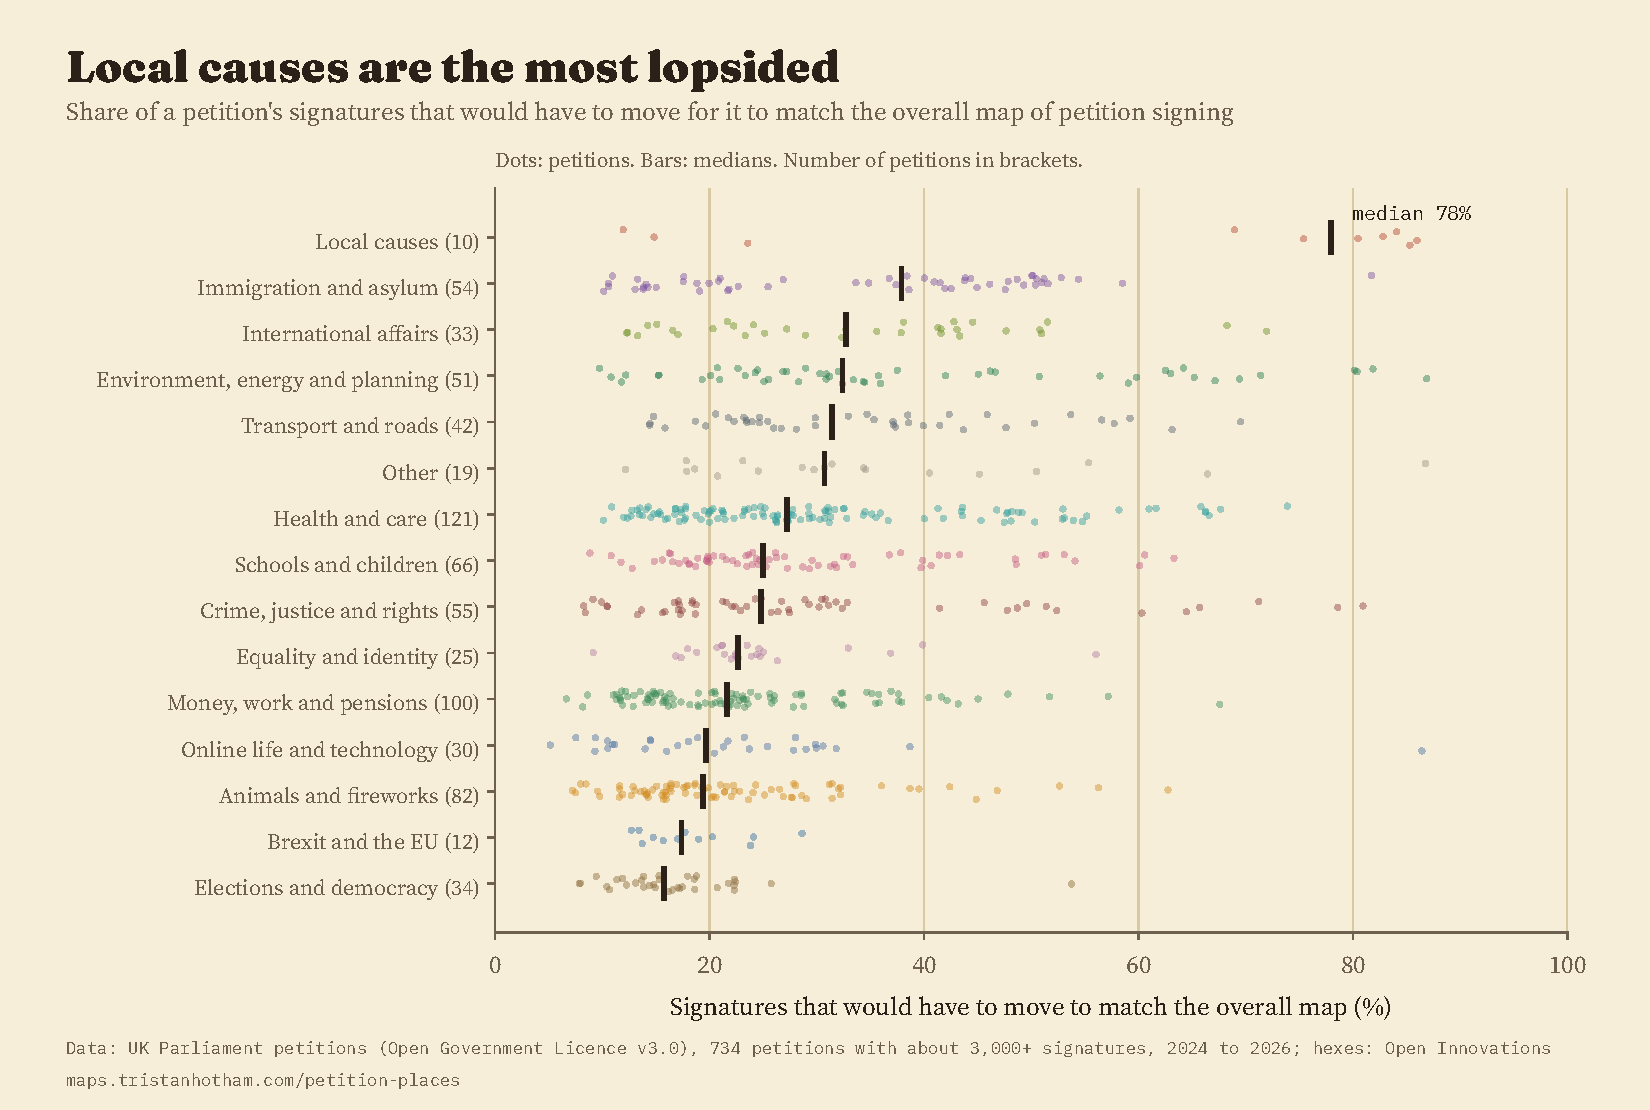
\includegraphics[width=0.92\textwidth]{f_family.pdf}\caption{Index of dissimilarity by topic family. Dots are petitions; bars are medians.}\label{fig:family}\end{figure}

\begin{table}[tbp]\centering\small\caption{H2: local causes against national petitions. OLS of log excess $D$ (floored at 0.005) on a local-cause indicator, log signatures and open status; HC3 errors. Entries: \% difference for local causes with 95\% CI.}\label{tab:h2}\begin{tabular}{lrrl}\toprule Specification & Petitions & Local & Local vs national (\%)\\\midrule
Main (final coding) & 734 & 10 & 189 [71, 389]\\
Keyword rules only & 734 & 25 & 152 [92, 231]\\
Petitions with 10,000+ signatures & 448 & 6 & 110 [$-$5, 365]\\
Petition-weighted $D$ (log $D$) & 734 & 10 & 107 [45, 195]\\
\bottomrule\end{tabular}\end{table}

\begin{figure}[tbp]\centering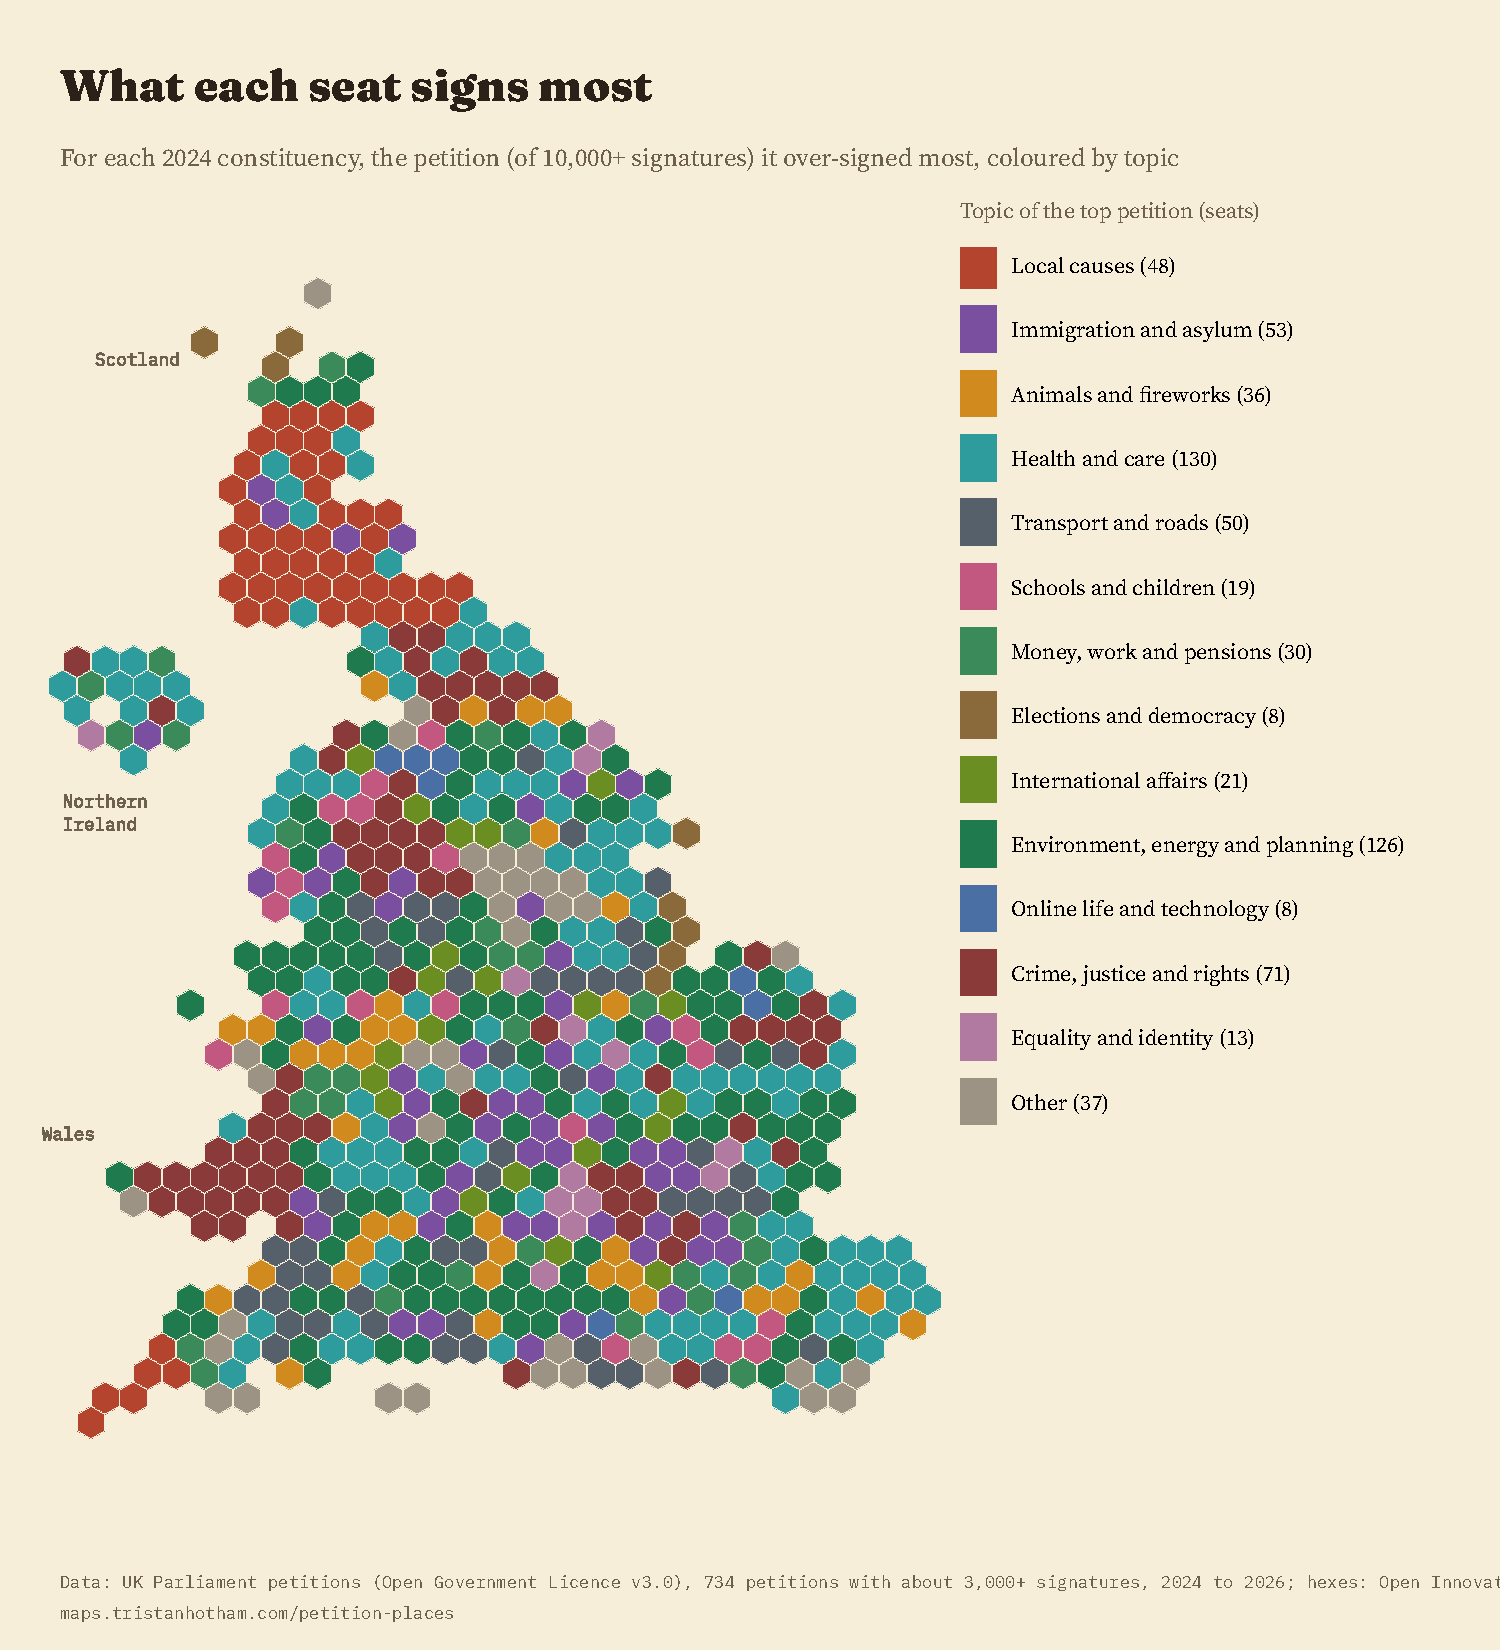
\includegraphics[width=0.78\textwidth]{f_top.pdf}\caption{Topic family of each seat's most over-signed petition (petitions with 10,000 or more signatures and at least 30 signatures in the seat). 144 different petitions top at least one seat.}\label{fig:top}\end{figure}

Figure~\ref{fig:top} maps the family of each seat's most over-signed petition among those with 10,000 or more signatures. Health petitions top 130 seats and environment and planning petitions 126; local causes top 48, mostly in Scotland and Cornwall. The most common single top petition is ``Hold a referendum on abolishing the Scottish Parliament \& Government'' (35 seats). The choice of top petition is the same with raw quotients in 98\% of seats.

\subsection{H3: two stable signature personalities}
The first principal component holds 20.2\% of the variation in the standardised log quotients, the second 9.8\% and the third 8.0\%; the first five together 44\% (Table~\ref{tab:pca}). Seat scores on the first component correlate 0.79 with the degree share, $-$0.72 with the share aged 65 and over, $-$0.76 with the White share and $-$0.67 with the Reform UK vote. The petitions loading most positively are about immigration routes, Gaza and Israel, and political donations; those loading most negatively are calls for a general election, offshore detention and penalties for social media posts. The second component separates Labour-held seats with poorer health (correlation with the Labour share 0.55, with poor health 0.39) from Conservative and Liberal Democrat seats with older populations (Conservative $-$0.54, Liberal Democrat $-$0.56, aged 65 and over $-$0.55); its most negative loadings are petitions on hares, climate and nature, farm animal cages, fossil fuel advertising and grouse shooting (Figure~\ref{fig:pca}).

The structure is stable. Computing the components separately for the 367 petitions created first and the 367 created later gives seat scores that correlate 0.96 on the first component, 0.96 on the second and 0.94 on the third. H3 is supported: the two leading components hold 30\% of the variation, above the planned 20\%, and stability exceeds the planned 0.7.

The silhouette width favours three groups of seats (0.37; four to eight groups score between 0.27 and 0.30). They are 450 seats of towns, suburbs and countryside in England and Wales; 124 seats in diverse cities (68 in London), where the mean degree share is 46\%; and 76 seats, 55 in Scotland, 18 in Northern Ireland and 3 in Wales (Figure~\ref{fig:clusters}). The third group probably partly reflects England-only petitions (school attendance fines, English bus passes), which residents of the devolved nations have little reason to sign.

\begin{figure}[tbp]\centering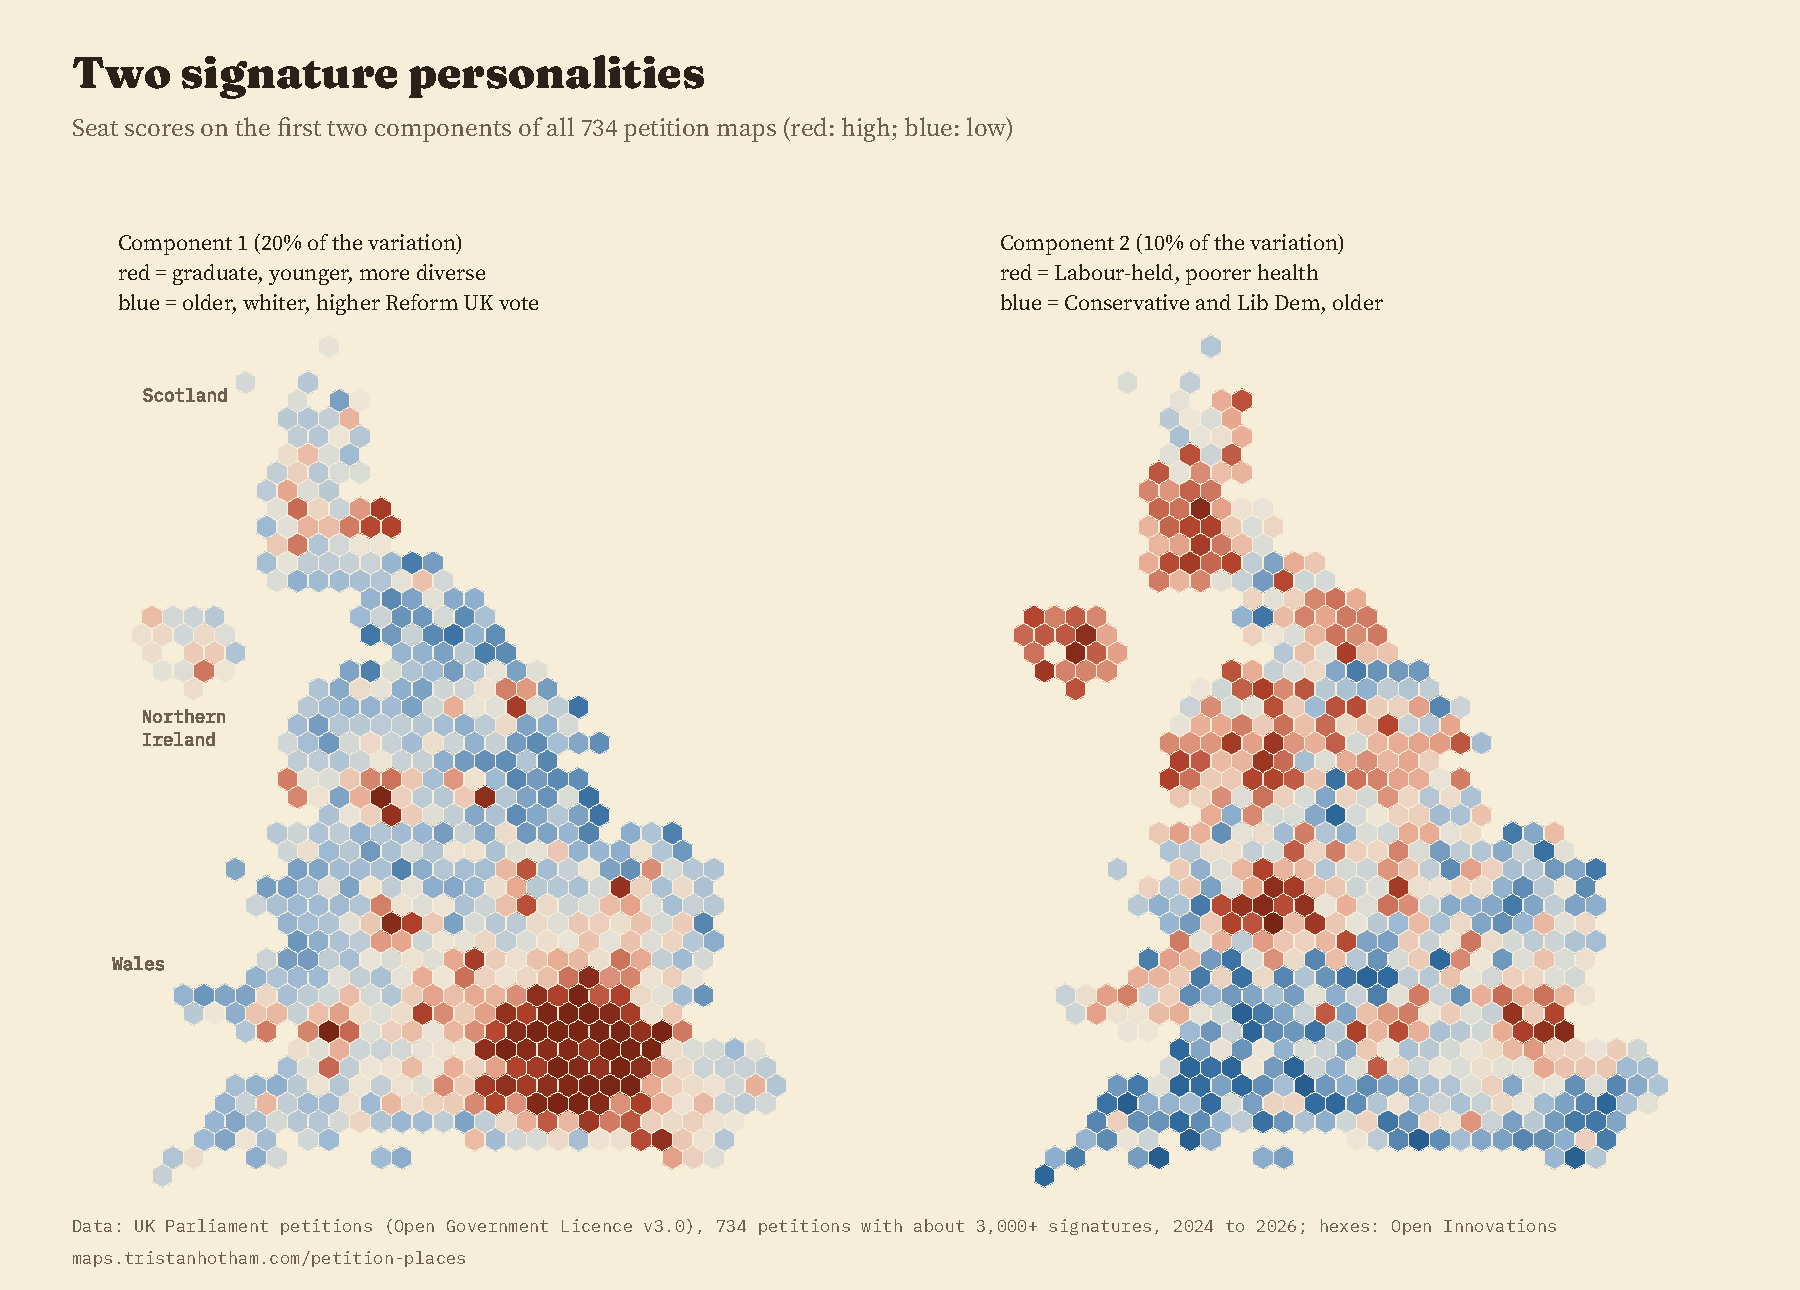
\includegraphics[width=\textwidth]{f_pca.pdf}\caption{Seat scores on the first two principal components of the 734 petition maps (standardised; red high, blue low).}\label{fig:pca}\end{figure}

\begin{table}[tbp]\centering\small\caption{H3: principal components of the seat-by-petition matrix of log location quotients. Correlations of seat scores with census shares ($N$ = 575 seats in England and Wales) and 2024 vote shares (Great Britain, $N$ = 632). Components oriented so that PC1 correlates positively with the degree share and PC2 with the Reform UK share.}\label{tab:pca}\begin{tabular}{lrrr}\toprule & PC1 & PC2 & PC3\\\midrule
Variance (\%) & 20.2 & 9.8 & 8.0\\
Split-half $r$ & 0.96 & 0.96 & 0.94\\\midrule
Degree & 0.79 & $-$0.43 & 0.26\\
Aged 65+ & $-$0.72 & $-$0.55 & 0.28\\
White & $-$0.76 & $-$0.49 & 0.36\\
Health not good & $-$0.69 & 0.39 & 0.14\\
Conservative & $-$0.31 & $-$0.54 & $-$0.38\\
Labour & 0.21 & 0.55 & 0.00\\
Liberal Democrat & 0.11 & $-$0.56 & 0.05\\
Reform UK & $-$0.67 & 0.15 & $-$0.42\\
Green & 0.49 & $-$0.04 & $-$0.02\\
Signatures per vote & $-$0.55 & 0.19 & $-$0.36\\
\bottomrule\end{tabular}\end{table}

\begin{figure}[tbp]\centering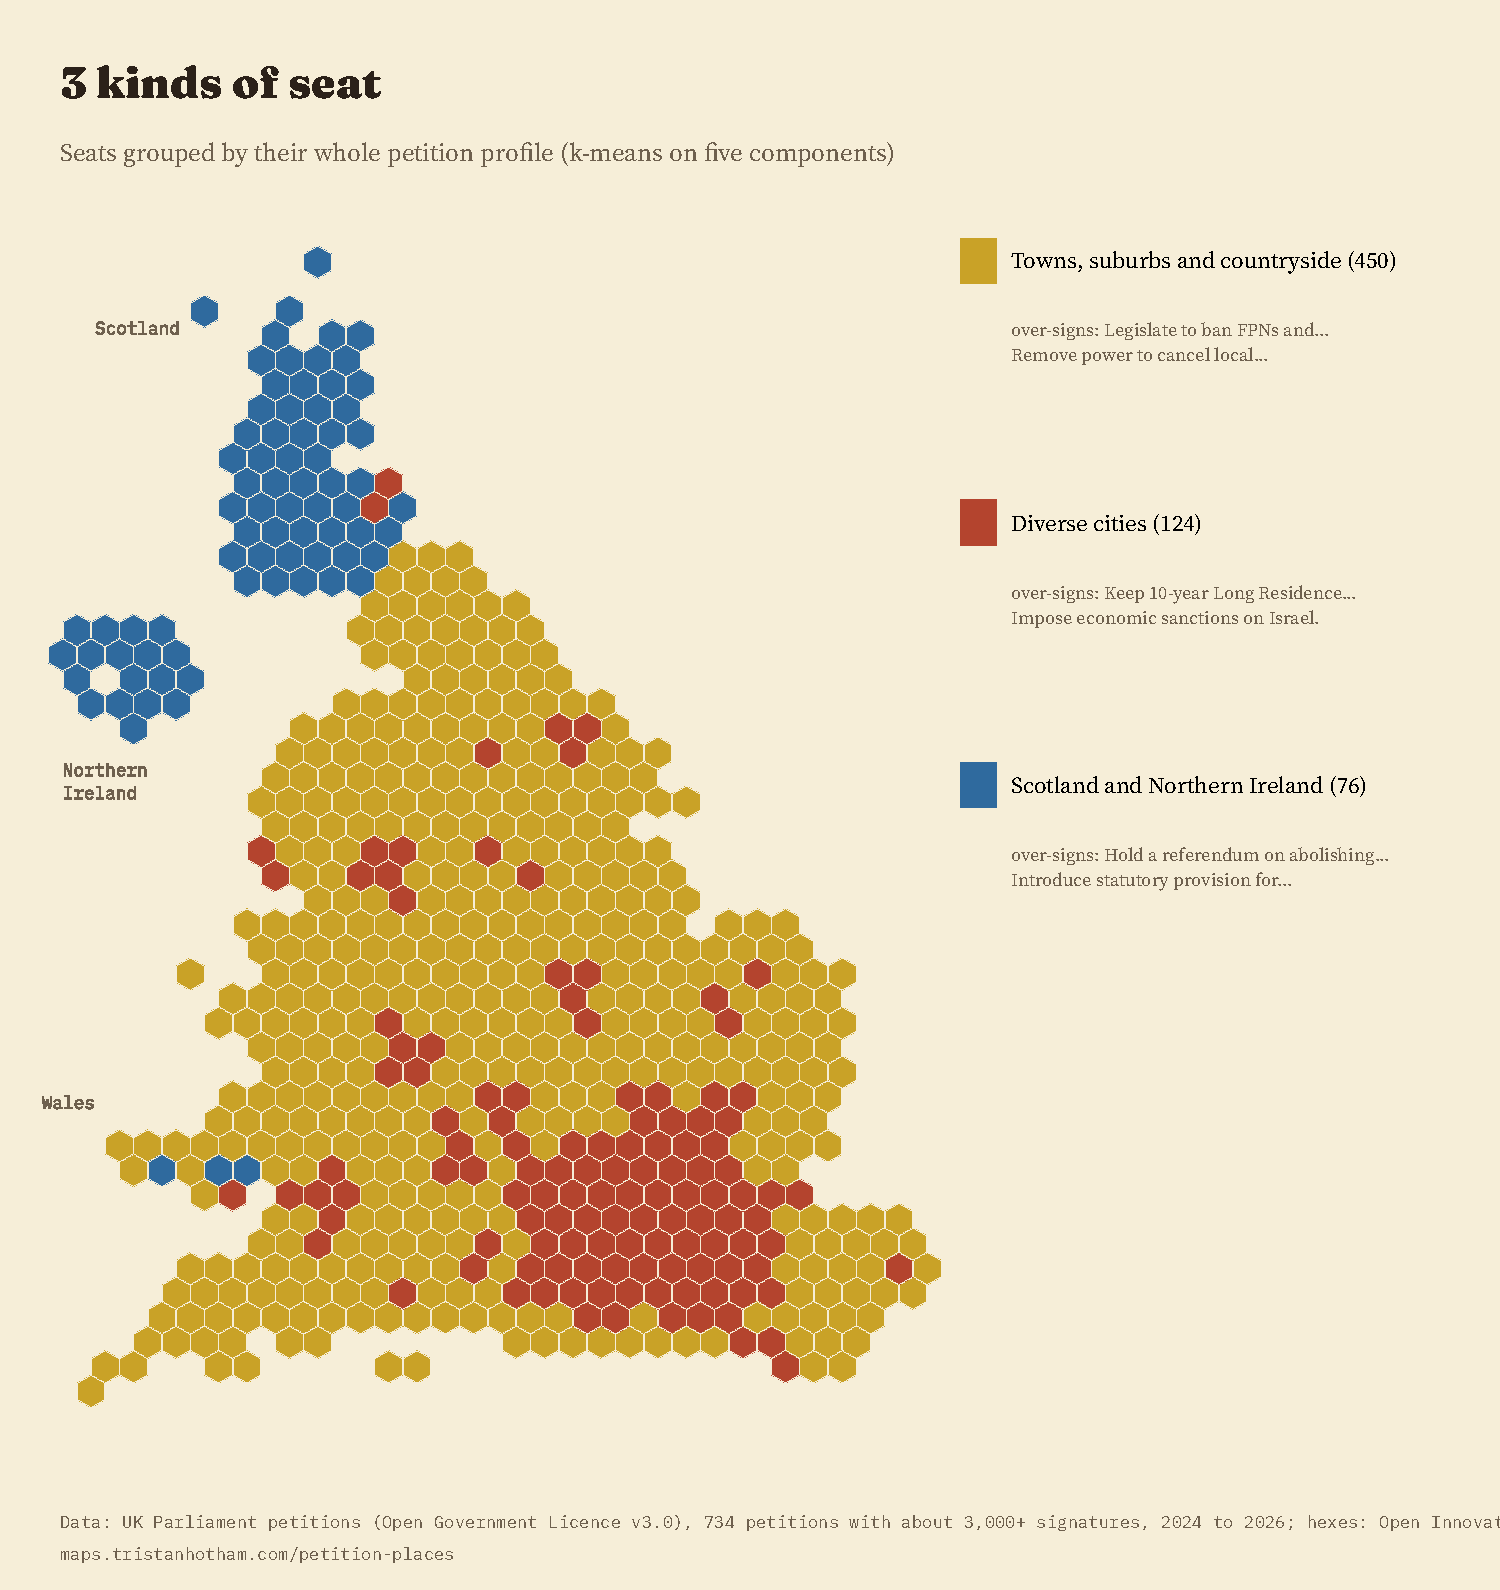
\includegraphics[width=0.78\textwidth]{f_clusters.pdf}\caption{Three groups of seats from $k$-means on the first five component scores ($k$ chosen by silhouette width).}\label{fig:clusters}\end{figure}

\subsection{H4: petition geography and the 2024 vote}\label{sec:votes}
Vote shares explain a median 26.3\% of the variance of a petition's map across the 632 seats of Great Britain (interquartile range 15\% to 38\%); 67 petitions exceed 50\%. Region fixed effects alone explain 25.7\% and the two together 39.6\%. With seats permuted, vote shares explain 0.9\%. In England and Wales, four census shares explain more than the six vote shares (median 31.2\% against 23.2\%; the vote does better for 17\% of petitions), and adding the vote to the census raises the median to 36.2\% (Table~\ref{tab:r2}, Figure~\ref{fig:votes}). The party whose share correlates most strongly with a petition's map is Reform UK for 345 petitions and the Conservatives for 169. The largest petition, ``Call a General Election'', is among those that follow the vote most closely ($R^2$ = 78\%; correlation with the Conservative share 0.69).

\begin{table}[tbp]\centering\small\caption{H4a: median share of variance in a petition's seat map explained, across the 734 petitions.}\label{tab:r2}\begin{tabular}{llr}\toprule Predictors & Seats & Median $R^2$ (\%)\\\midrule
Region fixed effects & GB (632) & 25.7\\
2024 vote shares (six parties) & GB (632) & 26.3\\
Vote shares and region & GB (632) & 39.6\\
Vote shares, seats permuted (placebo) & GB (632) & 0.9\\\midrule
Census shares (four) & E\&W (575) & 31.2\\
2024 vote shares & E\&W (575) & 23.2\\
Vote and census shares & E\&W (575) & 36.2\\
\bottomrule\end{tabular}\end{table}

For the directional tests (Table~\ref{tab:h4b}), EU petitions are under-signed where Reform UK polled well: $-$6.3\% per standard deviation (95\% CI $-$9.3 to $-$3.1), and over-signed where the Greens (3.6\%, CI 1.6 to 5.6) and the Liberal Democrats (3.7\%, CI 0.5 to 7.0) did well, holding census shares and region constant. The strongest single association of EU petitions is with the degree share (23.6\% per standard deviation). Immigration petitions as a family are over-signed where Reform UK polled well (3.6\%, CI 0.4 to 7.0), but are most strongly associated with a lower White share ($-$19.7\%). The directional expectations are therefore met in the main specification, but Section~\ref{sec:robust} shows that only the EU results are robust.

\begin{figure}[tbp]\centering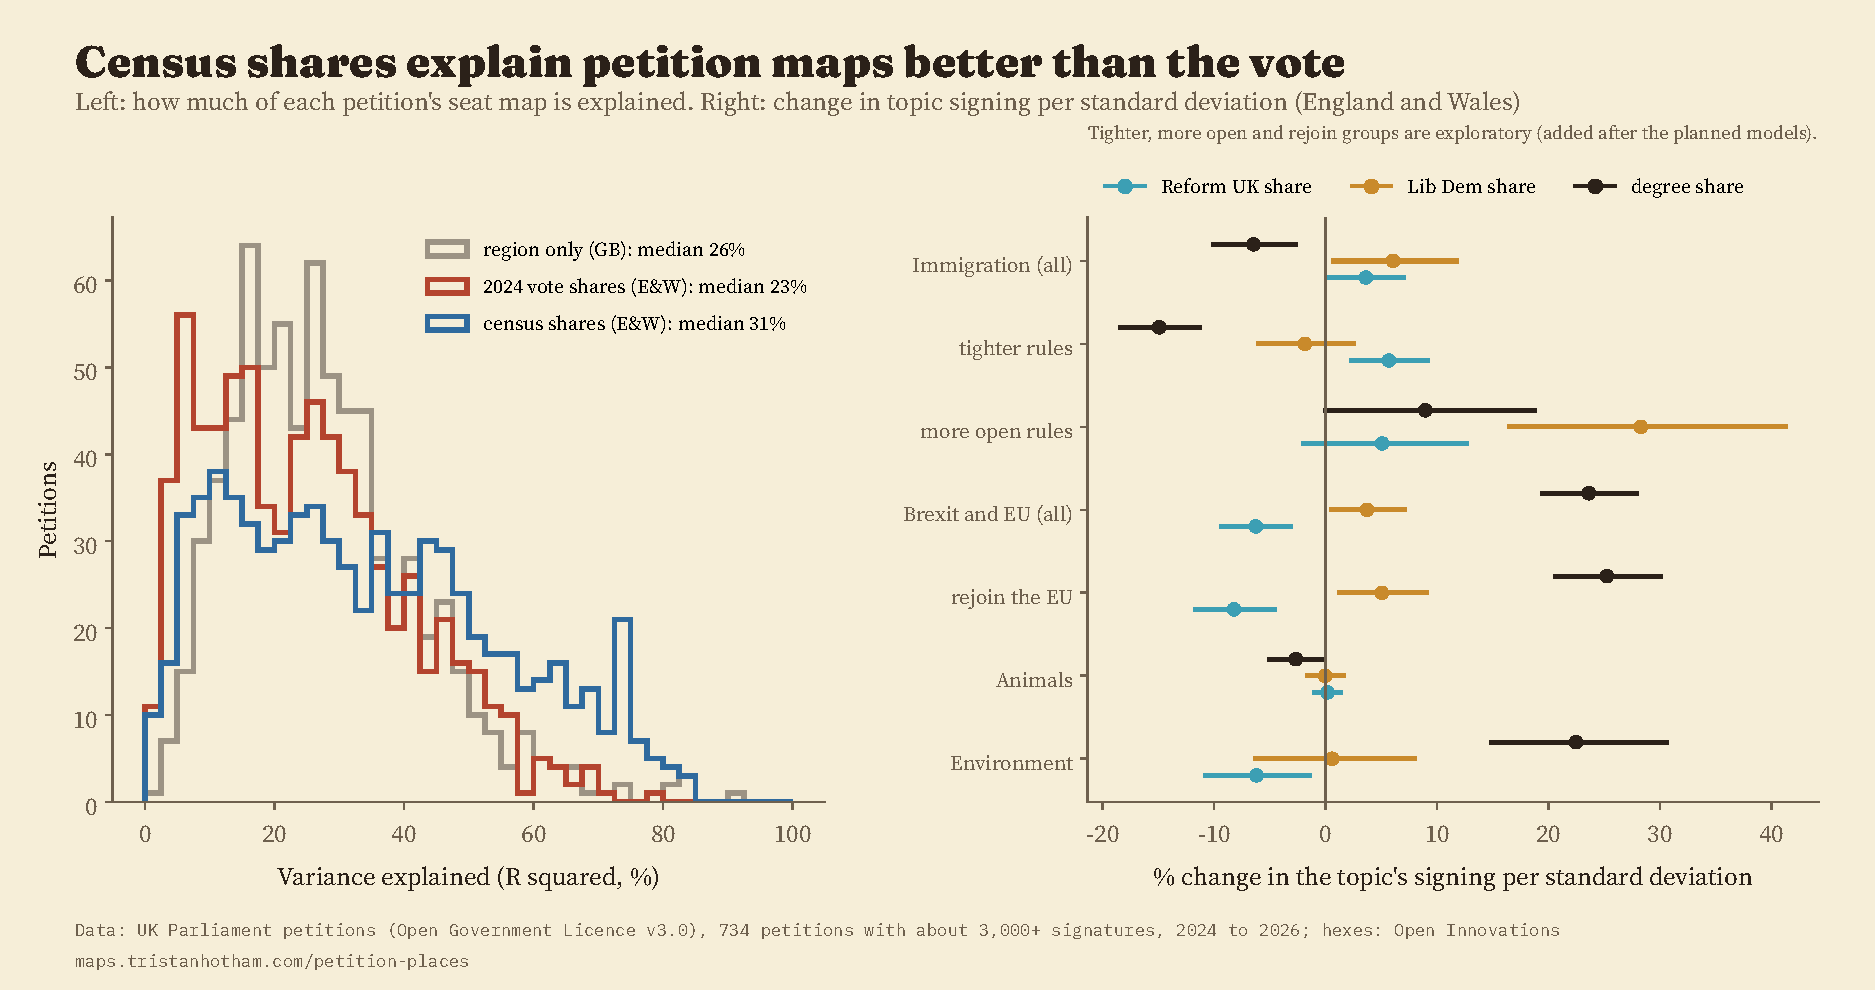
\includegraphics[width=\textwidth]{f_votes.pdf}\caption{Left: distribution of $R^2$ for each petition's map from region fixed effects (GB), 2024 vote shares and census shares (England and Wales). Right: percentage change in family over-signing per standard deviation of the Reform UK share, Liberal Democrat share and degree share, with 95\% CIs (England and Wales, census shares and region fixed effects). The tighter, more open and rejoin groups are exploratory.}\label{fig:votes}\end{figure}

\textbf{Exploratory.} After seeing the immigration result I split the family by stance, reading each title (Table~\ref{tab:expl}): 20 petitions ask for tighter rules and 33 ask to keep or open routes (mostly to settlement), one was ambiguous and left out. The two groups' seat maps correlate $-$0.56. Petitions for tighter rules are over-signed where Reform UK polled well (5.7\%, CI 2.3 to 9.1; map correlation 0.64) and in whiter seats; petitions to keep or open routes are over-signed in more diverse seats ($-$39.7\% per standard deviation of the White share) and where the Liberal Democrats and Labour did well. Restricting the EU family to the five rejoin petitions sharpens the EU result ($-$8.2\% for Reform UK, CI $-$11.7 to $-$4.6).

\section{Placebos and robustness}\label{sec:robust}
\subsection{Placebos}
Permuting seats removes the clustering (median $I$ $-$0.000) and the vote's explanatory power (median $R^2$ 0.9\%, close to the 1\% expected from six random regressors). The reliability check uses 21 groups of near-identical petitions (99 pairs; for example the six petitions calling for a general election, five on the personal allowance and five on rejoining the EU). Their maps correlate with a median of 0.63, against 0.01 for random pairs from different families; 85\% of the duplicate pairs exceed the 90th percentile of random pairs. The maps carry signal, not just noise.

\subsection{Alternative measures}
The clustering result does not depend on the measure: the median Moran's $I$ is 0.45 with six-nearest-neighbour weights, 0.50 with raw quotients, 0.48 with the petition-weighted denominator and 0.51 with valid votes. The local-cause contrast holds with the keyword rules alone (152\%, CI 92 to 231, with 25 petitions coded local) and with the petition-weighted dissimilarity (107\%, CI 45 to 195), but not among the larger petitions alone, as noted.

\subsection{The directional tests}
Table~\ref{tab:rob} and Figure~\ref{fig:robust} report the four directional estimates in 19 checks. The negative association of EU petitions with the Reform UK share holds in all 19 (range $-$8.4\% to $-$4.8\%). The positive association with the Green share holds in 18 and with the Liberal Democrat share in 15. The positive association of immigration petitions with the Reform UK share holds in only 10 of 19 and reverses sign without census controls ($-$6.8\%), so I do not treat it as robust.

\begin{figure}[tbp]\centering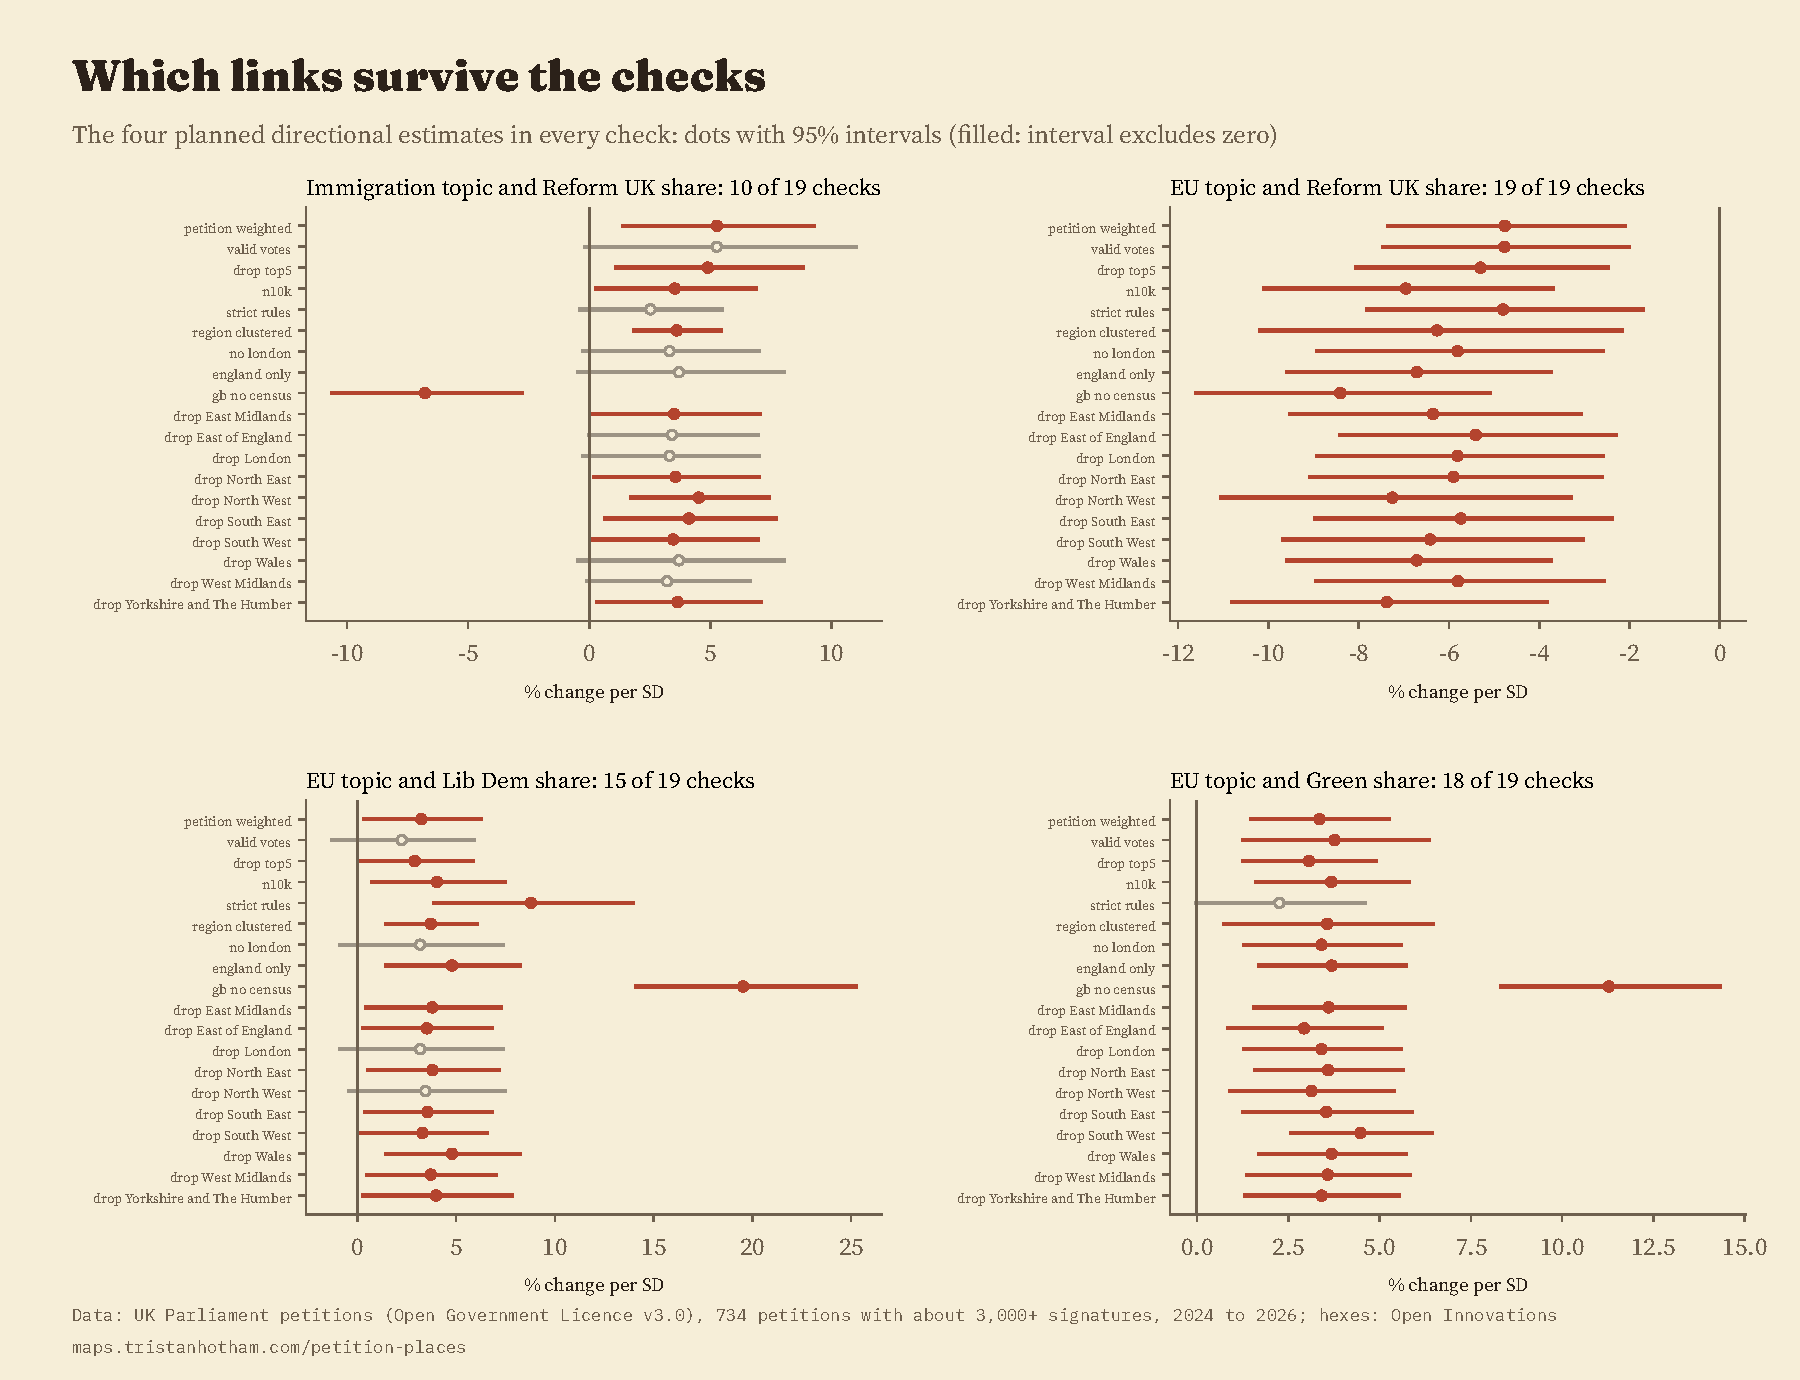
\includegraphics[width=\textwidth]{f_robust.pdf}\caption{The four directional estimates in every check (95\% CIs; filled where the interval excludes zero).}\label{fig:robust}\end{figure}

\begin{table}[tbp]\centering\scriptsize\caption{Robustness of the four directional estimates (\% change in family over-signing per SD, 95\% CI). Main: England and Wales, census shares and region fixed effects, HC3 errors.}\label{tab:rob}\setlength{\tabcolsep}{3pt}\begin{tabular}{lllll}\toprule Check & Immigration $\times$ Reform UK & EU $\times$ Reform UK & EU $\times$ Lib Dem & EU $\times$ Green\\\midrule
Main specification & 3.6 [0.4, 7.0] & $-$6.3 [$-$9.3, $-$3.1] & 3.7 [0.5, 7.0] & 3.6 [1.6, 5.6]\\\midrule
Petition-weighted denominator & 5.3 [1.4, 9.3] & $-$4.8 [$-$7.4, $-$2.1] & 3.2 [0.3, 6.2] & 3.4 [1.5, 5.3]\\
Valid votes denominator & 5.3 [$-$0.2, 11.0] & $-$4.8 [$-$7.5, $-$2.0] & 2.2 [$-$1.3, 5.9] & 3.8 [1.3, 6.3]\\
Five largest petitions dropped & 4.9 [1.1, 8.8] & $-$5.3 [$-$8.1, $-$2.5] & 2.9 [0.0, 5.9] & 3.1 [1.3, 4.9]\\
Petitions with 10,000+ signatures & 3.5 [0.3, 6.9] & $-$7.0 [$-$10.1, $-$3.7] & 4.0 [0.7, 7.4] & 3.7 [1.6, 5.8]\\
Keyword rules only & 2.5 [$-$0.4, 5.5] & $-$4.8 [$-$7.8, $-$1.7] & 8.8 [3.9, 13.9] & 2.3 [$-$0.0, 4.6]\\
Region-clustered errors & 3.6 [1.8, 5.4] & $-$6.3 [$-$10.2, $-$2.2] & 3.7 [1.5, 6.0] & 3.6 [0.7, 6.5]\\
London dropped & 3.3 [$-$0.2, 7.0] & $-$5.8 [$-$8.9, $-$2.6] & 3.2 [$-$0.8, 7.4] & 3.4 [1.3, 5.6]\\
England only & 3.7 [$-$0.5, 8.0] & $-$6.7 [$-$9.6, $-$3.7] & 4.8 [1.5, 8.2] & 3.7 [1.7, 5.7]\\
Great Britain, no census controls & $-$6.8 [$-$10.6, $-$2.8] & $-$8.4 [$-$11.6, $-$5.1] & 19.5 [14.1, 25.2] & 11.3 [8.3, 14.3]\\
Drop East Midlands & 3.5 [0.1, 7.0] & $-$6.4 [$-$9.5, $-$3.1] & 3.8 [0.4, 7.3] & 3.6 [1.6, 5.7]\\
Drop East of England & 3.4 [$-$0.0, 7.0] & $-$5.4 [$-$8.4, $-$2.3] & 3.5 [0.3, 6.8] & 2.9 [0.9, 5.1]\\
Drop London & 3.3 [$-$0.2, 7.0] & $-$5.8 [$-$8.9, $-$2.6] & 3.2 [$-$0.8, 7.4] & 3.4 [1.3, 5.6]\\
Drop North East & 3.6 [0.2, 7.0] & $-$5.9 [$-$9.1, $-$2.6] & 3.8 [0.5, 7.2] & 3.6 [1.6, 5.6]\\
Drop North West & 4.5 [1.7, 7.4] & $-$7.3 [$-$11.1, $-$3.3] & 3.4 [$-$0.4, 7.4] & 3.1 [0.9, 5.4]\\
Drop South East & 4.1 [0.6, 7.7] & $-$5.7 [$-$9.0, $-$2.4] & 3.5 [0.4, 6.8] & 3.5 [1.3, 5.9]\\
Drop South West & 3.5 [0.1, 7.0] & $-$6.4 [$-$9.7, $-$3.0] & 3.3 [0.1, 6.6] & 4.5 [2.6, 6.4]\\
Drop Wales & 3.7 [$-$0.5, 8.0] & $-$6.7 [$-$9.6, $-$3.7] & 4.8 [1.5, 8.2] & 3.7 [1.7, 5.7]\\
Drop West Midlands & 3.2 [$-$0.1, 6.6] & $-$5.8 [$-$8.9, $-$2.6] & 3.7 [0.5, 7.0] & 3.6 [1.4, 5.8]\\
Drop Yorkshire and The Humber & 3.7 [0.3, 7.1] & $-$7.4 [$-$10.8, $-$3.8] & 4.0 [0.3, 7.8] & 3.4 [1.3, 5.5]\\
\midrule Checks with CI excluding 0 & 10 of 19 & 19 of 19 & 15 of 19 & 18 of 19\\
\bottomrule\end{tabular}\end{table}

\section{Discussion}\label{sec:disc}
\subsection{What the maps show}
Petition signing is geographically structured in three ways. The first is simple: neighbouring places sign alike. Every petition map is clustered, which is what one would expect if signing spreads through local networks, local media and shared circumstances, and also what one would expect if the issues themselves are unevenly distributed. The second is that a minority of petitions are truly local. They come from places with a distinct identity or a concrete local project (Cornwall, Scotland, an East West Rail route) and their maps are nearly all in one place. That is the pattern MPs who worry about petitions bypassing constituencies \citep{matthews2021} might find most useful: such petitions are, in effect, constituency correspondence at scale.

The third and most consequential pattern is that national petitions share a small number of geographic dimensions. The first resembles the divide that runs through recent British electoral geography between graduate, younger and more diverse urban seats and older, whiter seats more open to Reform UK \citep{jenningsstoker2016,goodwinheath2016,beckeretal2017}. The second separates Labour-held seats with poorer health from Conservative and Liberal Democrat seats with older populations, and is marked by petitions on nature, the countryside and animal welfare. These dimensions are not party platforms. Petitions about animal welfare, health or the cost of living are signed across the political map, and the census describes petition geography better than the vote does. A plausible reading is that petition geography reflects who lives where, and what affects them, more than how they voted, but the design cannot separate these.

The second dimension deserves a cautious reading. Its negative pole gathers petitions on wildlife, the countryside, climate and animal welfare, and the seats that score low on it are older and more often held by Conservatives or Liberal Democrats; its positive pole gathers petitions on pay, benefits, carers and access to services in Labour-held seats with poorer health. One interpretation is that it separates concerns about the environment people live in from concerns about the means they live on. Another is that it partly reflects differences in which campaign organisations are active where. The data cannot decide between them, but the dimension is as stable as the first, which makes the organisational explanation less likely to be the whole story.

The near-perfect stability of the dimensions across independent sets of petitions is the strongest finding. It suggests that the maps record durable differences between places rather than the accidents of particular campaigns, and it gives some confidence that the dimensions identified here would reappear in later petitions. It also bears on a worry in the petitions literature, that a few high-volume petitions dominate the system \citep{jungherr2010}: because each petition's map is standardised before the components are extracted, every petition counts equally, and the same structure appears in the petitions created early and late in the Parliament.

The immigration result is a lesson in measurement. The planned test treated immigration petitions as one family and found a small association with the Reform UK vote that did not survive the checks. Reading the petitions suggests a reason: the family contains both petitions for tighter rules and petitions from people seeking to keep routes to settlement, and these have opposite geographies. Topic families that pool opposite positions can understate the link between petitions and politics. Future work could code stance systematically, as \citet{vidgen2020} and \citet{hagen2016} did for topics and language.

\subsection{Limitations}
The study is ecological. A seat that over-signs a petition contains more signers of that petition than expected, but the data cannot say whether they are the seat's voters for any particular party \citep{robinson1950}. Signing is a minority activity, unequal by education and age \citep{schlozman2010,escher2017}; measuring each petition against the seat's overall activity removes differences in the level of signing but not in who signs. Postcodes are self-reported. Some petitions were still open. Census controls cover England and Wales only, and the vote models leave out Northern Ireland, where different parties compete. Topic coding involved judgement; the overrides are published and the key results hold with the rules alone. The local-cause comparison rests on ten petitions. The hexagon map gives every seat equal area and so exaggerates rural seats' share of the national picture less than a real map would, but also distorts shapes; the real boundaries are provided as an alternative view.

\subsection{Implications}
For Parliament, the constituency counts already published could be summarised in the ways shown here, so that MPs and the Petitions Committee can see quickly whether a petition is national, local, or concentrated in a recognisable kind of place. For research, the petitions site offers a large and continuous record of issue salience at constituency level between elections, of the kind that \citet{jonesbaumgartner2005} and \citet{sorokawlezien2010} sought at national level and that representation research uses to judge how MPs relate to their constituents \citep{hanretty2017}.

\section{Conclusion}\label{sec:conc}
Every UK Parliament petition has a map, and the maps are not random. They cluster, they concentrate sharply for local causes, and they share two stable dimensions that mirror the education and age divides of British political geography. The 2024 vote accounts for about a quarter of a typical petition's map and census composition for a little more. The geography of what people petition about is a durable feature of places, visible between elections and seat by seat.

\section*{Data availability statement}
Data and code: Zenodo DOI https://doi.org/10.5281/zenodo.24104518. The interactive map is at \url{https://maps.tristanhotham.com/petition-places/} and the repository at \url{https://github.com/Tristan-Hotham/petition-places}. Petition data are from the UK Parliament petitions site (Open Government Licence v3.0); 2024 results, Census 2021 shares and simplified boundaries from voteReproject \citep{horan2025}; the hexagon layout from Open Innovations \citep{openinnovations2023}.

\section*{AI statement}
I wrote the text, with drafting and editing assistance from Claude (Anthropic), which also helped prepare the analysis code. I reviewed and checked all text and results.

\begin{thebibliography}{99}
\bibitem[Agnew(1987)]{agnew1987} Agnew, J. A. (1987) \textit{Place and Politics: The Geographical Mediation of State and Society}. Boston: Allen and Unwin.
\bibitem[Anselin(1995)]{anselin1995} Anselin, L. (1995) Local indicators of spatial association: LISA. \textit{Geographical Analysis} 27(2), 93 to 115. doi:10.1111/j.1538-4632.1995.tb00338.x.
\bibitem[Asher et al.(2019)]{asher2019} Asher, M., Leston-Bandeira, C. and Spaiser, V. (2019) Do parliamentary debates of e-petitions enhance public engagement with Parliament? An analysis of Twitter conversations. \textit{Policy and Internet} 11(2), 149 to 171. doi:10.1002/poi3.194.
\bibitem[Becker et al.(2017)]{beckeretal2017} Becker, S. O., Fetzer, T. and Novy, D. (2017) Who voted for Brexit? A comprehensive district-level analysis. \textit{Economic Policy} 32(92), 601 to 650. doi:10.1093/epolic/eix012.
\bibitem[Bochel(2013)]{bochel2013} Bochel, C. (2013) Petitions systems: contributing to representative democracy? \textit{Parliamentary Affairs} 66(4), 798 to 815.
\bibitem[Cameron and Miller(2015)]{cameronmiller2015} Cameron, A. C. and Miller, D. L. (2015) A practitioner's guide to cluster-robust inference. \textit{Journal of Human Resources} 50(2), 317 to 372.
\bibitem[Clayton and Kaldor(1987)]{claytonkaldor1987} Clayton, D. and Kaldor, J. (1987) Empirical Bayes estimates of age-standardized relative risks for use in disease mapping. \textit{Biometrics} 43(3), 671 to 681. doi:10.2307/2532003.
\bibitem[Duncan and Duncan(1955)]{duncan1955} Duncan, O. D. and Duncan, B. (1955) A methodological analysis of segregation indexes. \textit{American Sociological Review} 20(2), 210 to 217. doi:10.2307/2088328.
\bibitem[Escher and Riehm(2017)]{escher2017} Escher, T. and Riehm, U. (2017) Petitioning the German Bundestag: political equality and the role of the internet. \textit{Parliamentary Affairs} 70(1), 132 to 154. doi:10.1093/pa/gsw009.
\bibitem[Goodwin and Heath(2016)]{goodwinheath2016} Goodwin, M. J. and Heath, O. (2016) The 2016 referendum, Brexit and the left behind: an aggregate-level analysis of the result. \textit{Political Quarterly} 87(3), 323 to 332. doi:10.1111/1467-923X.12285.
\bibitem[Hagen et al.(2016)]{hagen2016} Hagen, L., Harrison, T. M., Uzuner, \"O., May, W., Fake, T. and Katragadda, S. (2016) E-petition popularity: do linguistic and semantic factors matter? \textit{Government Information Quarterly} 33(4), 783 to 795. doi:10.1016/j.giq.2016.07.006.
\bibitem[Hale et al.(2013)]{hale2013} Hale, S. A., Margetts, H. and Yasseri, T. (2013) Petition growth and success rates on the UK No. 10 Downing Street website. In \textit{Proceedings of the 5th Annual ACM Web Science Conference}. New York: ACM.
\bibitem[Halupka(2014)]{halupka2014} Halupka, M. (2014) Clicktivism: a systematic heuristic. \textit{Policy and Internet} 6(2), 115 to 132. doi:10.1002/1944-2866.POI355.
\bibitem[Hanretty et al.(2017)]{hanretty2017} Hanretty, C., Lauderdale, B. E. and Vivyan, N. (2017) Dyadic representation in a Westminster system. \textit{Legislative Studies Quarterly} 42(2), 235 to 267. doi:10.1111/lsq.12148.
\bibitem[Horan et al.(2025)]{horan2025} Horan, K., Domijan, K. and Brunsdon, C. (2025) voteReproject: preceding voting data reprojected to 2024 constituencies. R package, MIT licence. \url{https://github.com/horankev/voteReproject}.
\bibitem[Jennings and Stoker(2016)]{jenningsstoker2016} Jennings, W. and Stoker, G. (2016) The bifurcation of politics: two Englands. \textit{Political Quarterly} 87(3), 372 to 382. doi:10.1111/1467-923X.12228.
\bibitem[Johnston and Pattie(2006)]{johnstonpattie2006} Johnston, R. and Pattie, C. (2006) \textit{Putting Voters in Their Place: Geography and Elections in Great Britain}. Oxford: Oxford University Press.
\bibitem[Jolliffe and Cadima(2016)]{jolliffecadima2016} Jolliffe, I. T. and Cadima, J. (2016) Principal component analysis: a review and recent developments. \textit{Philosophical Transactions of the Royal Society A} 374, 20150202. doi:10.1098/rsta.2015.0202.
\bibitem[Jones and Baumgartner(2005)]{jonesbaumgartner2005} Jones, B. D. and Baumgartner, F. R. (2005) \textit{The Politics of Attention: How Government Prioritizes Problems}. Chicago: University of Chicago Press.
\bibitem[Jungherr and J\"urgens(2010)]{jungherr2010} Jungherr, A. and J\"urgens, P. (2010) The political click: political participation through e-petitions in Germany. \textit{Policy and Internet} 2(4), 131 to 165. doi:10.2202/1944-2866.1084.
\bibitem[Leston-Bandeira(2019)]{lestonbandeira2019} Leston-Bandeira, C. (2019) Parliamentary petitions and public engagement: an empirical analysis of the role of e-petitions. \textit{Policy and Politics} 47(3), 415 to 436. doi:10.1332/030557319X15579230420117.
\bibitem[MacKinnon and White(1985)]{mackinnon1985} MacKinnon, J. G. and White, H. (1985) Some heteroskedasticity-consistent covariance matrix estimators with improved finite sample properties. \textit{Journal of Econometrics} 29(3), 305 to 325.
\bibitem[Margetts et al.(2016)]{margetts2016} Margetts, H., John, P., Hale, S. and Yasseri, T. (2016) \textit{Political Turbulence: How Social Media Shape Collective Action}. Princeton: Princeton University Press.
\bibitem[Matthews(2021)]{matthews2021} Matthews, F. (2021) The value of `between-election' political participation: do parliamentary e-petitions matter to political elites? \textit{British Journal of Politics and International Relations} 23(3), 410 to 429. doi:10.1177/1369148120959041.
\bibitem[Moran(1950)]{moran1950} Moran, P. A. P. (1950) Notes on continuous stochastic phenomena. \textit{Biometrika} 37(1/2), 17 to 23. doi:10.1093/biomet/37.1-2.17.
\bibitem[Open Innovations(2023)]{openinnovations2023} Open Innovations (2023) UK constituencies 2023 hexmap (uk-constituencies-2023.hexjson), odileeds/hexmaps. MIT licence. \url{https://github.com/odileeds/hexmaps}.
\bibitem[Puschmann et al.(2017)]{puschmann2017} Puschmann, C., Bastos, M. T. and Schmidt, J.-H. (2017) Birds of a feather petition together? Characterizing e-petitioning through the lens of platform data. \textit{Information, Communication and Society} 20(2), 203 to 220. doi:10.1080/1369118X.2016.1162828.
\bibitem[Riehm et al.(2014)]{riehm2014} Riehm, U., B\"ohle, K. and Lindner, R. (2014) \textit{Electronic Petitioning and Modernization of Petitioning Systems in Europe}. Technology Assessment Studies Series 6. Berlin: Office of Technology Assessment at the German Bundestag (TAB).
\bibitem[Robinson(1950)]{robinson1950} Robinson, W. S. (1950) Ecological correlations and the behavior of individuals. \textit{American Sociological Review} 15(3), 351 to 357.
\bibitem[Rousseeuw(1987)]{rousseeuw1987} Rousseeuw, P. J. (1987) Silhouettes: a graphical aid to the interpretation and validation of cluster analysis. \textit{Journal of Computational and Applied Mathematics} 20, 53 to 65. doi:10.1016/0377-0427(87)90125-7.
\bibitem[Schlozman et al.(2010)]{schlozman2010} Schlozman, K. L., Verba, S. and Brady, H. E. (2010) Weapon of the strong? Participatory inequality and the internet. \textit{Perspectives on Politics} 8(2), 487 to 509. doi:10.1017/S1537592710001210.
\bibitem[Seabold and Perktold(2010)]{seabold2010} Seabold, S. and Perktold, J. (2010) statsmodels: econometric and statistical modeling with Python. In \textit{Proceedings of the 9th Python in Science Conference}, 92 to 96.
\bibitem[Soroka and Wlezien(2010)]{sorokawlezien2010} Soroka, S. N. and Wlezien, C. (2010) \textit{Degrees of Democracy: Politics, Public Opinion, and Policy}. Cambridge: Cambridge University Press.
\bibitem[UK Parliament(2026)]{petitions2026} UK Parliament (2026) Petitions: UK Government and Parliament. \url{https://petition.parliament.uk/}, retrieved 2026. Open Government Licence v3.0.
\bibitem[Vidgen and Yasseri(2020)]{vidgen2020} Vidgen, B. and Yasseri, T. (2020) What, when and where of petitions submitted to the UK government during a time of chaos. \textit{Policy Sciences} 53(3), 535 to 557. doi:10.1007/s11077-020-09395-y.
\bibitem[Wright(2012)]{wright2012} Wright, S. (2012) Assessing (e-)democratic innovations: ``democratic goods'' and Downing Street e-petitions. \textit{Journal of Information Technology and Politics} 9(4), 453 to 470. doi:10.1080/19331681.2012.712820.
\bibitem[Wright(2016)]{wright2016} Wright, S. (2016) `Success' and online political participation: the case of Downing Street e-petitions. \textit{Information, Communication and Society} 19(6), 843 to 857. doi:10.1080/1369118X.2015.1080285.
\bibitem[Yasseri et al.(2017)]{yasseri2017} Yasseri, T., Hale, S. A. and Margetts, H. Z. (2017) Rapid rise and decay in petition signing. \textit{EPJ Data Science} 6, 20. doi:10.1140/epjds/s13688-017-0116-6.
\end{thebibliography}

\clearpage
\appendix
\section{Appendix: full tables and data construction}
\subsection{Data construction}
The constituency counts were matched to the 650 GSS codes of the hexagon layout and the voteReproject data; all codes match. Seats with no signatures for a petition are absent from the site's lists and were set to zero. Contiguity: polygons simplified to about 150 metres were buffered by about 250 metres and intersected; Na h-Eileanan an Iar and Orkney and Shetland were linked to their nearest seat; Northern Ireland seats are neighbours only of each other. The empirical Bayes shape parameter was estimated separately for each petition. The topic overrides, the stance coding used in the exploratory analysis and the near-identical petition groups are listed in the code.

\begin{table}[tbp]\centering\scriptsize\caption{H4b: family over-signing on 2024 vote shares and census shares (England and Wales, $N$ = 575 seats, region fixed effects, HC3). Entries: \% change per SD; $^{*}$ 95\% CI excludes zero. Con, Lab, LD, Ref, Grn: Conservative, Labour, Liberal Democrat, Reform UK and Green shares; 65+, Deg, Hlth, White: census shares aged 65 and over, degree or higher, health not good, White. Full estimates with standard errors are in data/models.csv.}\label{tab:h4b}\setlength{\tabcolsep}{3pt}\begin{tabular}{lrrrrrrrrrr}\toprule Family & Con & Lab & LD & Ref & Grn & 65+ & Deg & Hlth & White & $R^2$ (\%)\\\midrule
Local causes & 7.3$^{*}$ & $-$6.3$^{*}$ & $-$5.4 & 4.1$^{*}$ & $-$6.7$^{*}$ & 4.0 & 3.5 & 2.4 & 13.6$^{*}$ & 56\\
Immigration and asylum & 4.8$^{*}$ & 5.0 & 6.1$^{*}$ & 3.6$^{*}$ & $-$0.2 & $-$10.4$^{*}$ & $-$6.5$^{*}$ & 1.3 & $-$19.7$^{*}$ & 69\\
Brexit and the EU & $-$6.6$^{*}$ & 7.0$^{*}$ & 3.7$^{*}$ & $-$6.3$^{*}$ & 3.6$^{*}$ & 11.6$^{*}$ & 23.6$^{*}$ & 2.4 & 3.9$^{*}$ & 80\\
Animals and fireworks & $-$1.1 & 0.3 & $-$0.0 & 0.2 & 0.3 & 5.4$^{*}$ & $-$2.7$^{*}$ & $-$4.6$^{*}$ & 9.7$^{*}$ & 70\\
Health and care & $-$3.0$^{*}$ & 4.0$^{*}$ & 0.9 & $-$1.0 & 0.6 & $-$0.1 & $-$2.6 & $-$7.2$^{*}$ & 6.2$^{*}$ & 29\\
Transport and roads & $-$1.6 & $-$1.3 & 1.8 & 2.6 & $-$1.3 & 5.8$^{*}$ & $-$11.9$^{*}$ & $-$12.3$^{*}$ & $-$0.1 & 37\\
Schools and children & 0.3 & 2.1 & 2.2 & $-$0.8 & $-$3.4$^{*}$ & $-$5.4$^{*}$ & $-$5.5$^{*}$ & $-$4.8$^{*}$ & 4.1$^{*}$ & 59\\
Money, work and pensions & $-$0.2 & 2.8$^{*}$ & 0.1 & $-$0.1 & $-$1.2 & 7.6$^{*}$ & $-$4.0$^{*}$ & $-$3.4$^{*}$ & $-$0.5 & 46\\
Elections and democracy & 5.3$^{*}$ & $-$3.9$^{*}$ & $-$2.7$^{*}$ & 3.6$^{*}$ & $-$1.7$^{*}$ & $-$0.2 & $-$3.0$^{*}$ & $-$0.6 & 9.6$^{*}$ & 89\\
International affairs & $-$9.1$^{*}$ & $-$6.5 & $-$6.0 & $-$9.0$^{*}$ & 2.4 & 2.2 & 39.6$^{*}$ & 13.8$^{*}$ & $-$37.9$^{*}$ & 90\\
Environment, energy and planning & $-$7.1$^{*}$ & $-$0.4 & 0.6 & $-$6.2$^{*}$ & 6.5$^{*}$ & 21.2$^{*}$ & 22.5$^{*}$ & $-$2.9 & 15.9$^{*}$ & 65\\
Online life and technology & $-$0.3 & 0.3 & $-$0.1 & $-$0.3 & $-$0.1 & $-$7.2$^{*}$ & 0.3 & 4.6$^{*}$ & 3.9$^{*}$ & 57\\
Crime, justice and rights & 6.0$^{*}$ & $-$2.2 & $-$0.2 & 3.4$^{*}$ & $-$1.0 & $-$6.3$^{*}$ & $-$2.6 & 6.6$^{*}$ & 9.4$^{*}$ & 71\\
Equality and identity & $-$0.7 & 10.5$^{*}$ & 7.4$^{*}$ & $-$3.3$^{*}$ & 10.2$^{*}$ & $-$6.5$^{*}$ & 20.8$^{*}$ & 7.1$^{*}$ & $-$0.6 & 73\\
Other & $-$7.0$^{*}$ & 4.4 & 4.4 & $-$6.0 & $-$1.0 & 12.0$^{*}$ & $-$1.3 & 4.2 & 6.9$^{*}$ & 42\\
\bottomrule\end{tabular}\end{table}

\begin{table}[tbp]\centering\scriptsize\caption{Exploratory (added after the planned models): the H4b model for immigration petitions split by stance and for the rejoin petitions alone. Number of petitions in brackets. Notation as in Table~\ref{tab:h4b}.}\label{tab:expl}\setlength{\tabcolsep}{3pt}\begin{tabular}{lrrrrrrrrrr}\toprule Group & Con & Lab & LD & Ref & Grn & 65+ & Deg & Hlth & White & $R^2$ (\%)\\\midrule
Immigration: tighter rules (20) & 5.4$^{*}$ & $-$2.7 & $-$1.9 & 5.7$^{*}$ & $-$4.9$^{*}$ & $-$4.2$^{*}$ & $-$14.9$^{*}$ & $-$0.9 & 15.0$^{*}$ & 84\\
Immigration: keep or open routes (33) & 10.2$^{*}$ & 21.5$^{*}$ & 28.3$^{*}$ & 5.1 & 3.2 & $-$36.2$^{*}$ & 8.9 & 5.8 & $-$39.7$^{*}$ & 81\\
EU: rejoin (5) & $-$8.3$^{*}$ & 8.9$^{*}$ & 5.0$^{*}$ & $-$8.2$^{*}$ & 4.4$^{*}$ & 14.0$^{*}$ & 25.2$^{*}$ & 1.3 & 1.7 & 81\\
\bottomrule\end{tabular}\end{table}

\end{document}
